\documentclass[a4paper,12pt]{article}

\usepackage[utf8]{inputenc}
\usepackage[T1]{fontenc}
\usepackage[french]{babel}
\usepackage{graphicx}
\usepackage{geometry}
\usepackage{array}
\usepackage{booktabs}
\usepackage{listings}
\usepackage{xcolor}
\usepackage{hyperref}
\usepackage{enumitem}
\usepackage{fancyhdr}
\usepackage{titlesec}
\usepackage{fontawesome5}
\usepackage{float} % Indispensable pour l'option [H] des figures

\geometry{margin=2.5cm}

\definecolor{codebg}{rgb}{0.95,0.95,0.95}
\definecolor{codeframe}{rgb}{0.7,0.7,0.7}
\definecolor{bleu}{RGB}{30,90,180}

\lstset{
  backgroundcolor=\color{codebg},
  frame=single,
  rulecolor=\color{codeframe},
  basicstyle=\ttfamily\small,
  breaklines=true,
  showstringspaces=false,
  language=PHP,
  keywordstyle=\color{bleu}\bfseries,
  commentstyle=\color{gray}\itshape,
  stringstyle=\color{red!70!black},
}

\pagestyle{fancy}
\fancyhf{}
\rhead{Projet ÉVASION – L2 MIASHS MIAGE}
\lhead{\leftmark}
\rfoot{\thepage}

\hypersetup{
  colorlinks=true,
  linkcolor=bleu,
  urlcolor=bleu,
}

\begin{document}

% --- PAGE DE GARDE ---
\begin{titlepage}
    \centering
    \vspace*{1cm}
    
    
\includegraphics[width=6cm]{logo.png}\\[1cm] 
    
    {\Huge \textbf{ÉVASION}}\\[0.4cm]
    {\large Rapport de projet –}\\[0.2cm]
    {\large Plateforme web de découverte et de réservation de voyages}\\[1cm]
    
    \rule{\linewidth}{0.8pt}\\[2cm]

    \begin{minipage}{0.45\textwidth}
        \centering
        \textbf{Yahou Sarah}\\
        {\small n° étudiant : 45011767}\\[0.2cm]
        \href{https://github.com/sarahyahou}{\faGithub \ GitHub Sarah}
    \end{minipage}
    \hfill
    \begin{minipage}{0.45\textwidth}
        \centering
        \textbf{Kebbache Walid}\\
        {\small n° étudiant : 45003317}\\[0.2cm]
        \href{https://github.com/PRIXOOO}{\faGithub \ GitHub Walid}
    \end{minipage}

    \vfill

    {\large L2 MIASHS parcours MIAGE}\\[0.2cm]
    {\large Université Paris Nanterre}\\[0.5cm]
    \rule{4cm}{0.4pt}\\[0.5cm]
    \today
\end{titlepage}

\newpage
\tableofcontents
\newpage

% ---------------------------------------------------------
\section{Introduction}

Dans le cadre de nos enseignements de L2 MIASHS parcours MIAGE, nous avons réalisé \textbf{ÉVASION}, un site web dynamique simulant une agence de voyages en ligne.

L'objectif du projet était de maîtriser le développement web full-stack en intégrant plusieurs technologies complémentaires :

\begin{itemize}
  \item \textbf{PHP} (back-end, gestion des sessions, traitement des formulaires)
  \item \textbf{MySQL / MariaDB} (persistance des données via PDO)
  \item \textbf{HTML / CSS / JavaScript} (interface utilisateur responsive)
  \item \textbf{JSON} (format d'échange avec l'API d'IA)
  \item \textbf{API Mistral AI} (\texttt{mistral-large-latest}) pour la recommandation
  \item \textbf{API Pixabay} pour chercher des images avec des mots clés
\end{itemize}

Ce rapport détaille la conception, l'architecture technique, les fonctionnalités implémentées ainsi que les difficultés rencontrées au cours du développement.

% ---------------------------------------------------------
\section{Présentation du site}

\textbf{ÉVASION} est une plateforme permettant à des utilisateurs connectés de découvrir des destinations de voyage et de constituer leur liste de réservations personnelles. Le point central du site est une page d'accueil dynamique avec un système d'onglets (vols, hôtels, découverte par IA).

\subsection{Rôles des utilisateurs}

\begin{description}
  \item[Utilisateur non connecté] Peut consulter la page d'accueil et les destinations mises en avant, mais doit s'inscrire ou se connecter pour réserver.
  \item[Utilisateur connecté] Peut accéder à l'ensemble des fonctionnalités : recherche IA, réservation, gestion de son profil.
\end{description}

\subsection{Particularité : l'assistant IA}

L'utilisateur formule sa demande en langage naturel. L'IA de \textbf{Mistral AI}(\texttt{mistral-large-latest}) génère alors de manière autonome un voyage personnalisé complet (titre, pays, dates, prix, description) sans piocher dans un catalogue préexistant. La réponse est ensuite affichée sur une page dédiée avec une image récupérée via l'\textbf{API Pixabay}.

% ---------------------------------------------------------
\section{Fonctionnalités}

Voici l'ensemble des fonctionnalités implémentées dans le projet :

\begin{itemize}
  \item \textbf{Accueil dynamique} : page d'accueil avec section héro, onglets interactifs (Vol, Hôtel, Découverte IA), carrousel de témoignages animé et autocomplétion des villes via l'API Open-Meteo.
  \item \textbf{Inscription} : création d'un compte utilisateur avec validation des champs et hachage du mot de passe (\texttt{password\_hash}).
  \item \textbf{Authentification} : connexion sécurisée avec vérification du mot de passe haché (\texttt{password\_verify}) et gestion de session PHP.
  \item \textbf{Déconnexion} : destruction de la session (\texttt{session\_destroy}).
  \item \textbf{Recherche IA} : envoi d'un prompt en langage naturel à l'API Mistral AI via cURL~; la réponse JSON est décodée et affichée avec la destination recommandée.
  \item \textbf{Gestion des réservations} : ajout d'un voyage au panier (stocké en session), affichage de la liste des voyages réservés avec calcul du coût total, suppression d'une réservation (\texttt{DELETE}).
  \item \textbf{Profil utilisateur} :
    \begin{itemize}
      \item Mise à jour du nom et de l'e-mail
      \item Changement du mot de passe (vérification de l'ancien avant mise à jour)
      \item Upload d'une photo de profil (JPG, PNG, GIF) renommée selon l'ID utilisateur
      \item Suppression définitive du compte (suppression BDD + fichier image)
    \end{itemize}
  \item \textbf{Interface responsive} : menu hamburger pour mobile avec animation CSS, sous-menu profil déroulant.
\end{itemize}

% ---------------------------------------------------------
\section{Conception}

\subsection{Diagramme de cas d'utilisation}

\textbf{Acteurs :}
\begin{itemize}
  \item \textbf{Visiteur} : utilisateur non authentifié
  \item \textbf{Utilisateur connecté} : dispose d'un compte actif
\end{itemize}

\textbf{Cas d'utilisation principaux :}

\begin{center}
\begin{tabular}{|l|l|}
\hline
\textbf{Acteur} & \textbf{Cas d'utilisation} \\
\hline
Visiteur & Consulter l'accueil, S'inscrire, Se connecter \\
\hline
Utilisateur connecté & Rechercher par IA, Réserver un voyage, \\
 & Voir ses réservations, Gérer son profil, Se déconnecter \\
\hline
\end{tabular}
\end{center}

\vspace{0.5cm}

\begin{figure}[H]
    \centering
    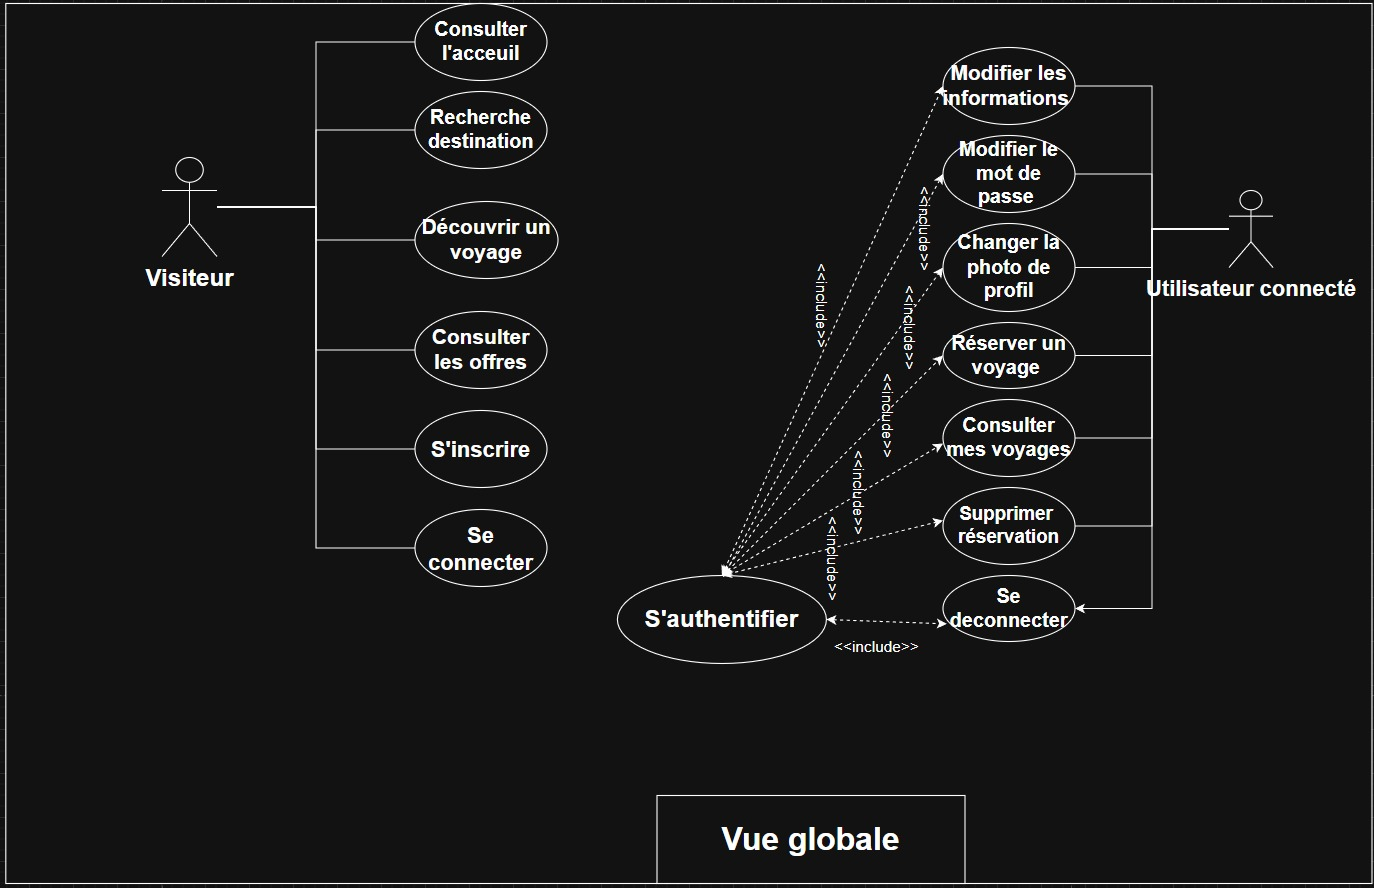
\includegraphics[width=\textwidth]{vue_globale.jpeg}
    \caption{Diagramme des cas d'utilisation globale}
\end{figure}

\begin{figure}[H]
    \centering
    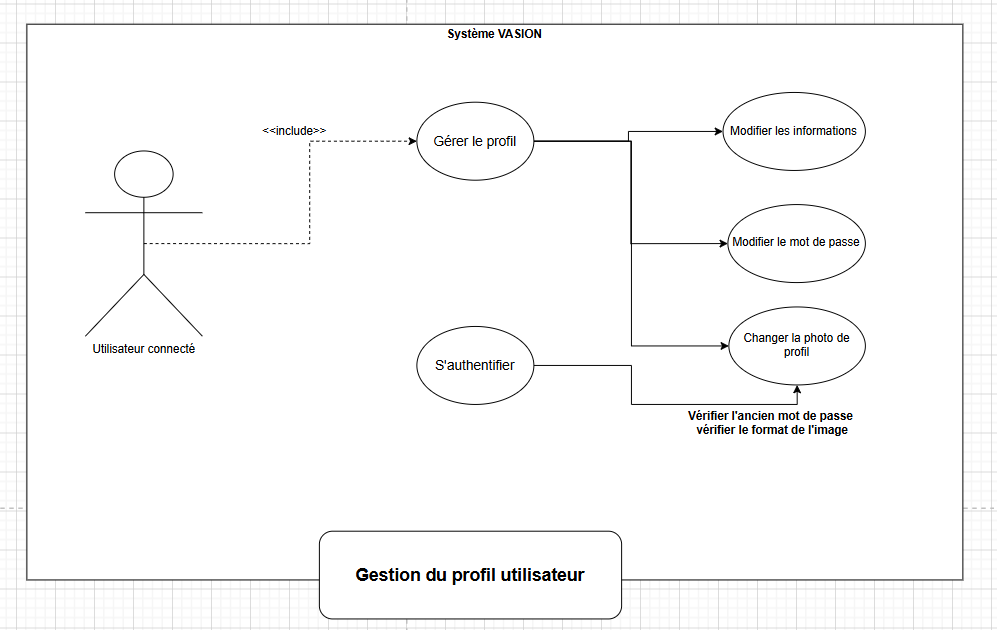
\includegraphics[width=0.8\textwidth]{img_Gestion_profil_utilisateur.png}
    \caption{Cas d'utilisation - Gestion du profil}
\end{figure}

\begin{figure}[H]
    \centering
    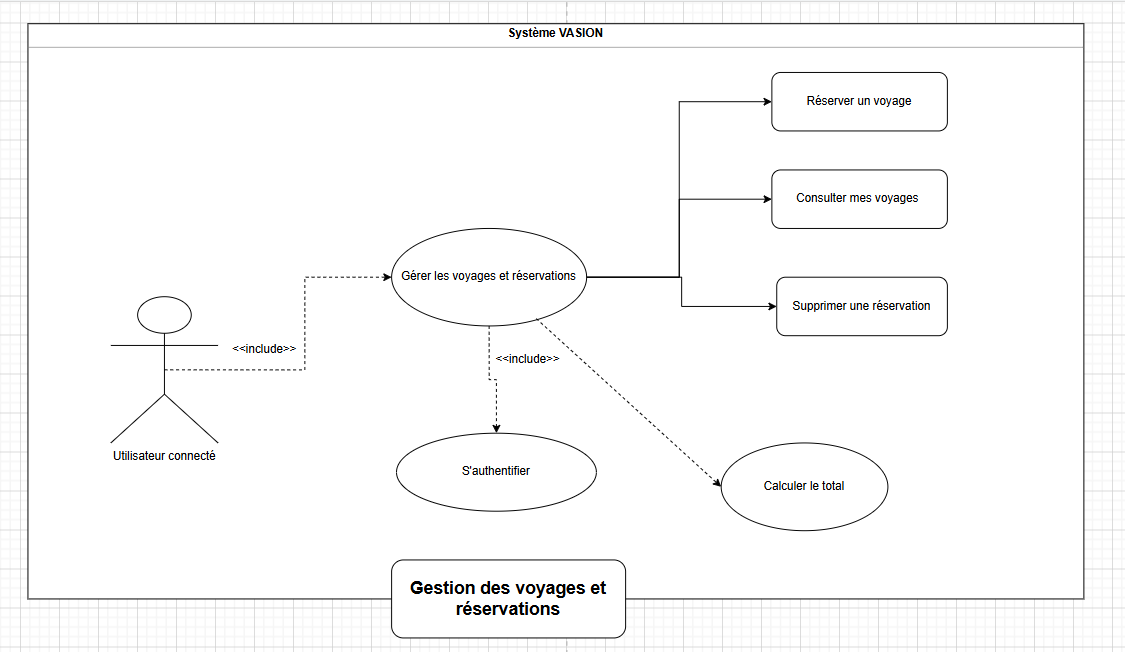
\includegraphics[width=0.8\textwidth]{img_Gestion_Voyages_Reservation.png}
    \caption{Cas d'utilisation - Réservation}
\end{figure}

\begin{figure}[H]
    \centering
    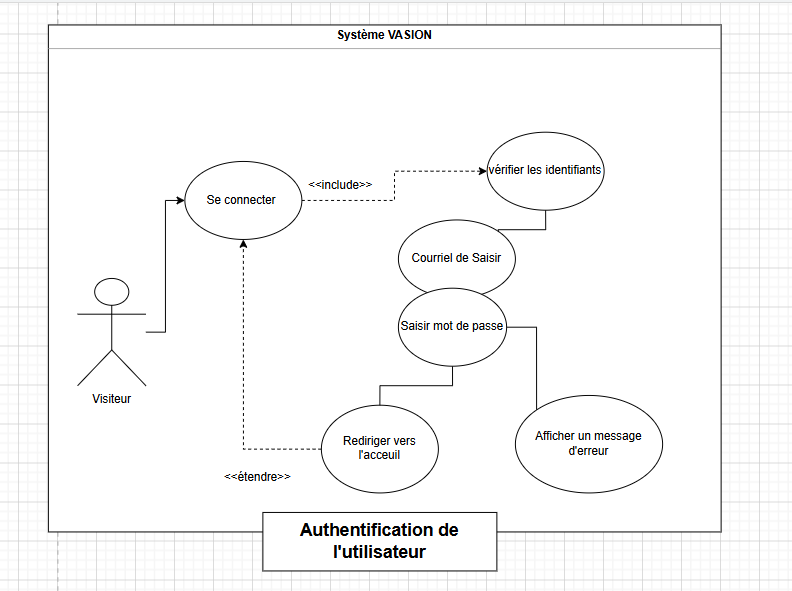
\includegraphics[width=0.8\textwidth]{img_Authentification_utilisateur.png}
    \caption{Cas d'utilisation - Authentification}
\end{figure}

\subsection{Diagramme de classes UML}

\begin{figure}[H]
    \centering
    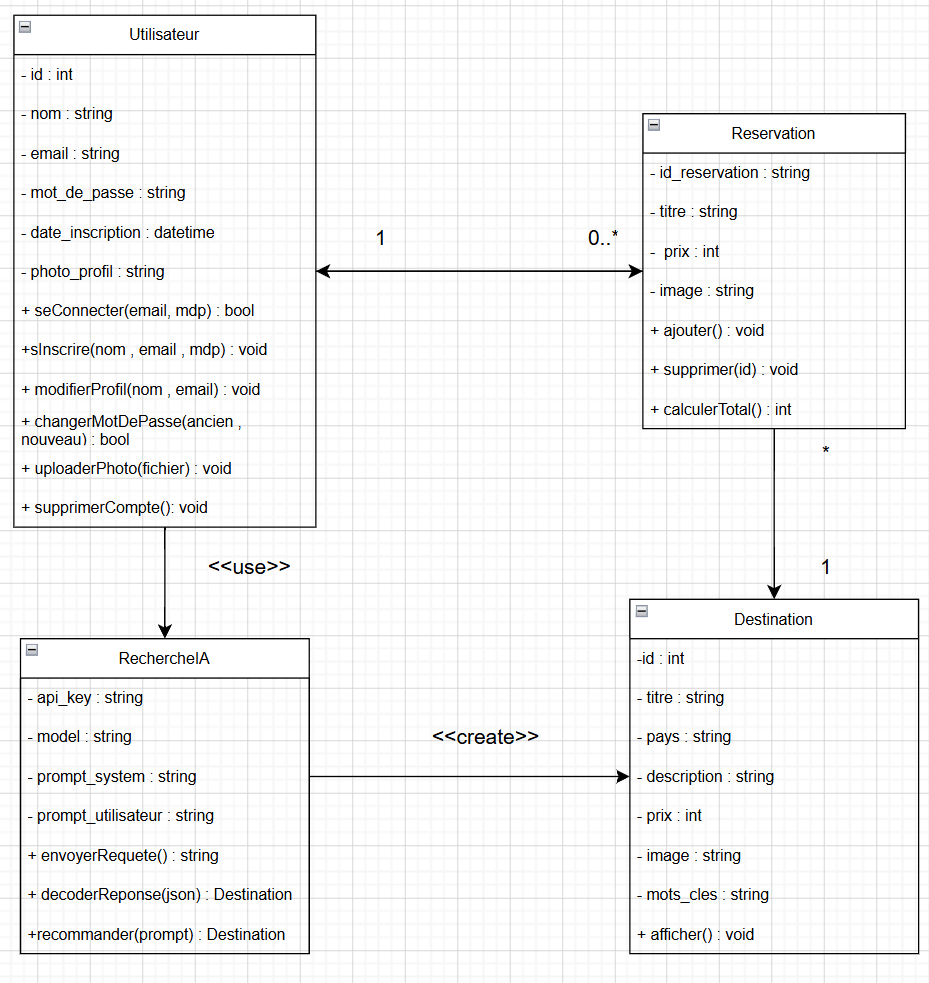
\includegraphics[width=\textwidth]{diagramme_classes_UML_officiel.png}
    \caption{Diagramme de classes du système ÉVASION}
\end{figure}

\paragraph{Description des entités :}

\begin{table}[H]
\centering
\begin{tabular}{|p{3cm}|p{10cm}|}
\hline
\textbf{Classe} & \textbf{Description} \\
\hline
\texttt{Utilisateur} & Représente tout utilisateur du système (visiteur, client connecté). Contient les informations d'authentification et de profil. \\
\hline
\texttt{Destination} & Entité représentant une offre de voyage (titre, pays, description, prix, image, mots-clés). \\
\hline
\texttt{Reservation} & Entité temporaire stockée en session représentant l'ajout d'une destination au panier par un utilisateur. \\
\hline
\end{tabular}
\caption{Description des classes principales}
\end{table}

\paragraph{Relations :}

\begin{itemize}
    \item \textbf{Association 1,n} : Un \texttt{Utilisateur} peut avoir 0 à plusieurs \texttt{Reservations} (panier).
    \item \textbf{Association 1,n} : Une \texttt{Destination} peut être réservée 0 à plusieurs fois.
    \item \textbf{Héritage} : Dans une version évoluée, \texttt{Visiteur} hériterait de \texttt{Utilisateur}. Un rôle \texttt{Administrateur} pourrait également être ajouté.
\end{itemize}

\paragraph{Contraintes techniques actuelles :}
Les réservations sont actuellement stockées en session PHP et non persistées en base de données. Une table \texttt{reservations} serait nécessaire pour une version professionnelle.

\subsection{Diagramme de séquence}

\textbf{Exemple : recherche d'une destination par IA}

\begin{enumerate}
    \item L'utilisateur saisit une description en langage naturel dans l'onglet \og Découverte\fg{}.
    \item Le navigateur soumet le formulaire en \texttt{POST} vers \texttt{recherche\_ia.php}.
    \item Le script PHP construit un prompt système fixe qui décrit le format de réponse attendu, et l'associe au prompt utilisateur saisi.
    \item Une requête cURL est envoyée à l'API Mistral AI (\texttt{mistral-large-latest}) avec \texttt{response\_format: json\_object}.
    \item L'API retourne un objet JSON contenant le voyage généré (titre, pays, prix, dates, description).
    \item PHP appelle l'API Pixabay pour récupérer une illustration correspondant au pays.
    \item La page affiche la destination recommandée avec son image et un bouton \og Réserver\fg{}.
\end{enumerate}

\begin{figure}[H]
    \centering
    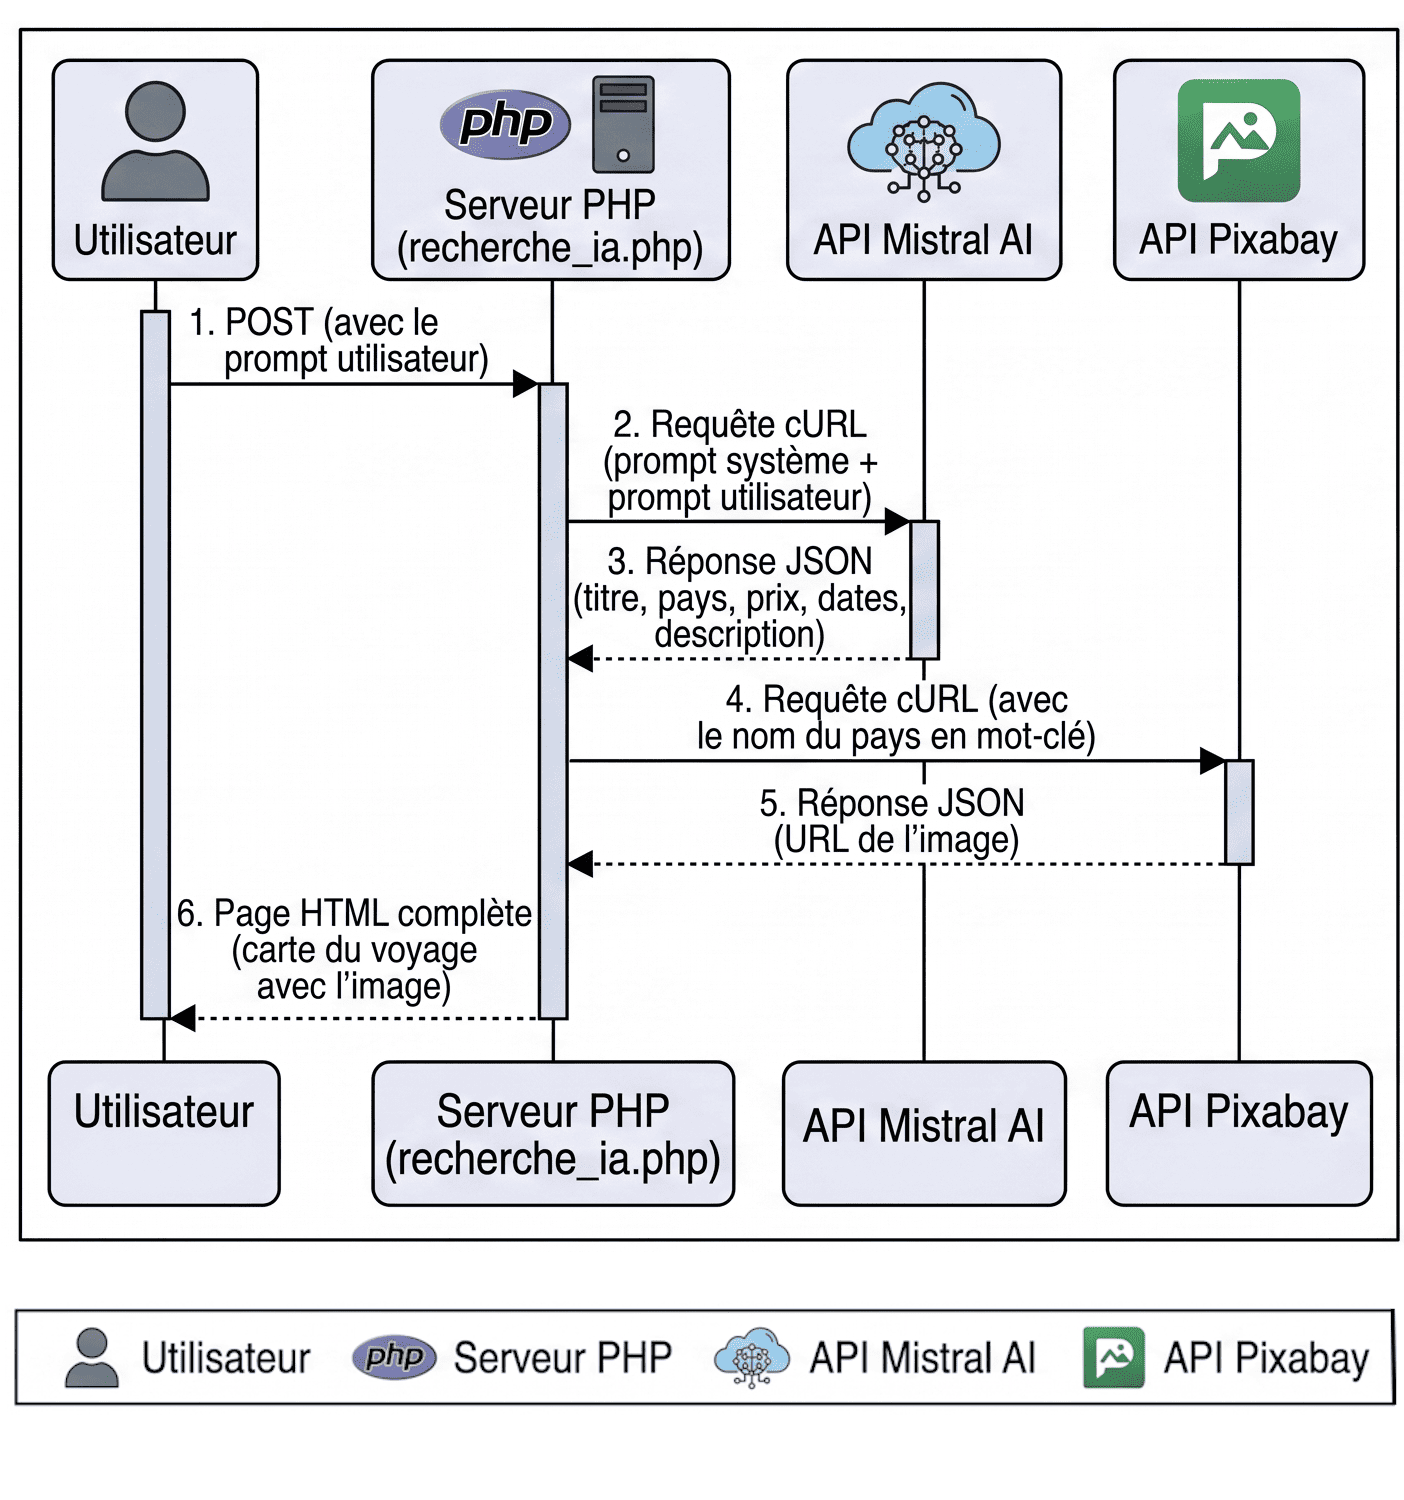
\includegraphics[width=\textwidth]{Diagrammeseq1.png}
    \caption{Diagramme de séquence de la recherche IA}
\end{figure}

\begin{figure}[H]
    \centering
    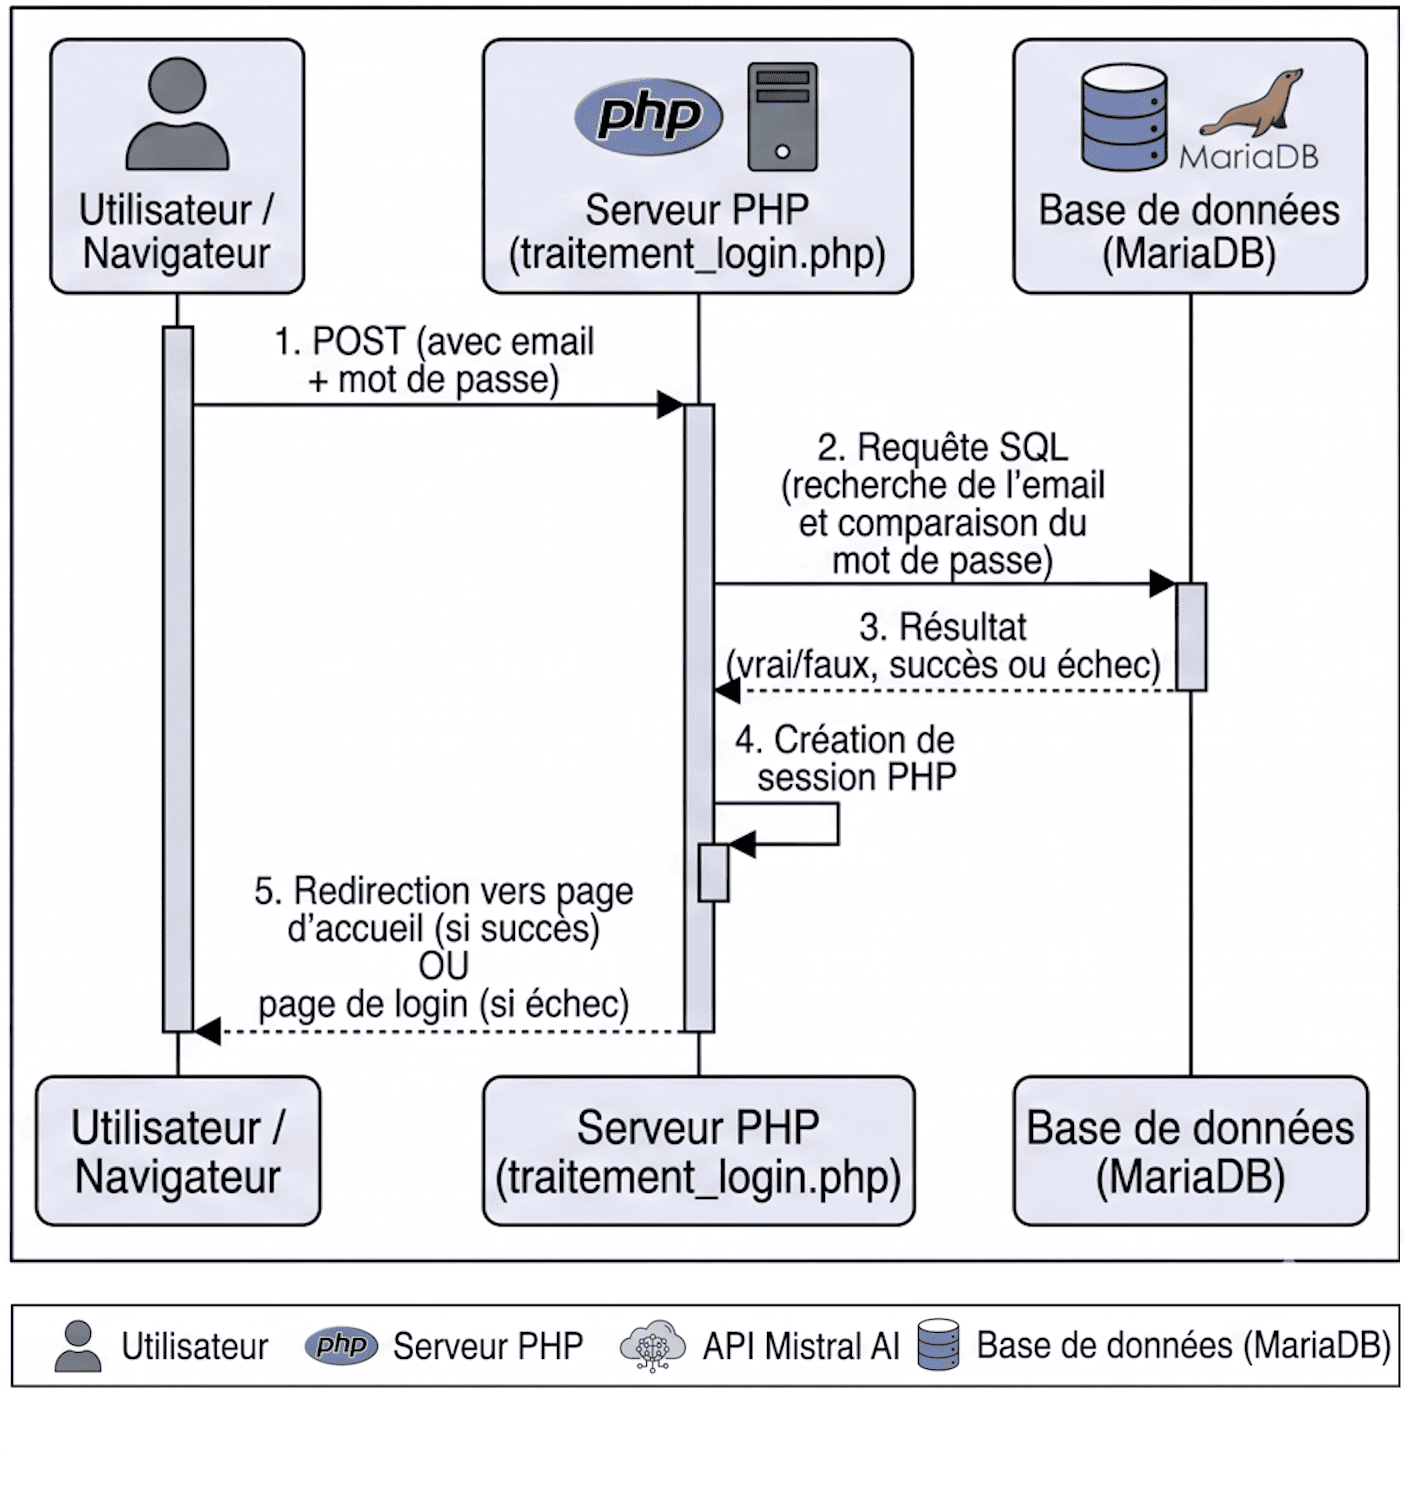
\includegraphics[width=\textwidth]{Diagrammeseq2.png}
    \caption{Diagramme de séquence de l'Authentification Utilisateur}
\end{figure}
\subsection{Description détaillée des cas d'utilisation}

% --- Cas 1 : Inscription ---
\subsubsection*{1. Inscription (\texttt{register.php})}
\begin{itemize}[label=\textbullet]
    \item \textbf{Objectif :} Permettre à un visiteur de créer un compte pour accéder aux fonctionnalités de réservation.
    \item \textbf{Acteur concerné :} Visiteur.
    \item \textbf{Préconditions :} L'utilisateur n'est pas authentifié.
    \item \textbf{Scénario nominal :}
    \begin{enumerate}[label=\arabic*.]
        \item Le visiteur accède à la page d'inscription.
        \item Il remplit le formulaire (nom, email, mot de passe).
        \item Il soumet le formulaire.
        \item Le système vérifie que l'adresse e-mail n'est pas déjà utilisée en base de données.
        \item Le système hache le mot de passe (\texttt{password\_hash}) et enregistre le nouvel utilisateur.
    \end{enumerate}
    \item \textbf{Postconditions :} Le compte est créé, l'utilisateur est redirigé vers la page de connexion avec un message de succès.
\end{itemize}

\vspace{0.3cm}

% --- Cas 2 : Connexion ---
\subsubsection*{2. Connexion (\texttt{login.php})}
\begin{itemize}[label=\textbullet]
    \item \textbf{Objectif :} Authentifier un utilisateur pour lui donner accès à son espace personnel.
    \item \textbf{Acteur concerné :} Visiteur (possédant déjà un compte).
    \item \textbf{Préconditions :} L'utilisateur possède un compte valide et n'est pas connecté.
    \item \textbf{Scénario nominal :}
    \begin{enumerate}[label=\arabic*.]
        \item L'utilisateur accède à la page de connexion.
        \item Il saisit son adresse e-mail et son mot de passe.
        \item Il valide le formulaire.
        \item Le système recherche l'e-mail en base et vérifie la correspondance du mot de passe (\texttt{password\_verify}).
        \item Le système initialise la session utilisateur (\texttt{\$\_SESSION}).
    \end{enumerate}
    \item \textbf{Postconditions :} L'utilisateur est authentifié et redirigé vers la page d'accueil.
\end{itemize}

\vspace{0.3cm}

% --- Cas 3 : Recherche IA ---
\subsubsection*{3. Recherche IA (\texttt{recherche\_ia.php})}
\begin{itemize}[label=\textbullet]
    \item \textbf{Objectif :} Générer une proposition de voyage sur mesure à partir d'une requête en langage naturel.
    \item \textbf{Acteur concerné :} Utilisateur connecté.
    \item \textbf{Préconditions :} L'utilisateur est authentifié.
    \item \textbf{Scénario nominal :}
    \begin{enumerate}[label=\arabic*.]
        \item L'utilisateur saisit ses critères de voyage dans le champ de découverte IA.
        \item Il soumet sa demande.
        \item Le système construit un prompt structuré et l'envoie à l'API Mistral AI.
        \item L'API retourne les détails du voyage généré au format JSON.
        \item Le système interroge l'API Pixabay avec le pays généré pour récupérer une image illustrative.
        \item Le système affiche la proposition complète avec un bouton de réservation.
    \end{enumerate}
    \item \textbf{Postconditions :} Une destination personnalisée est affichée à l'écran, prête à être réservée.
\end{itemize}

\vspace{0.3cm}

% --- Cas 4 : Ajout d'un voyage au panier ---
\subsubsection*{4. Ajout d'un voyage au panier (\texttt{voyages.php})}
\begin{itemize}[label=\textbullet]
    \item \textbf{Objectif :} Sauvegarder une destination en vue d'une réservation.
    \item \textbf{Acteur concerné :} Utilisateur connecté.
    \item \textbf{Préconditions :} L'utilisateur est authentifié et consulte une offre de voyage.
    \item \textbf{Scénario nominal :}
    \begin{enumerate}[label=\arabic*.]
        \item L'utilisateur clique sur le bouton \og Réserver \fg{} d'une destination.
        \item Le système récupère les informations du voyage (titre, pays, prix).
        \item Le système génère un identifiant unique (\texttt{uniqid()}) pour cette réservation.
        \item Le système ajoute ces informations au tableau \texttt{\$\_SESSION['panier']}.
        \item Le système redirige l'utilisateur vers la page de ses réservations.
    \end{enumerate}
    \item \textbf{Postconditions :} Le voyage est enregistré dans la session courante de l'utilisateur et le coût total est mis à jour.
\end{itemize}

\vspace{0.3cm}

% --- Cas 5 : Gestion du profil ---
\subsubsection*{5. Gestion du profil (\texttt{profil.php})}
\begin{itemize}[label=\textbullet]
    \item \textbf{Objectif :} Consulter et mettre à jour les informations personnelles du compte.
    \item \textbf{Acteur concerné :} Utilisateur connecté.
    \item \textbf{Préconditions :} L'utilisateur est authentifié.
    \item \textbf{Scénario nominal :}
    \begin{enumerate}[label=\arabic*.]
        \item L'utilisateur accède à la page de son profil.
        \item Il modifie les champs souhaités (nom, e-mail) ou téléverse une nouvelle photo de profil.
        \item Il soumet le formulaire de mise à jour.
        \item Le système vérifie la validité des données (et l'extension du fichier image si applicable).
        \item Le système met à jour la base de données et enregistre la nouvelle image sur le serveur.
    \end{enumerate}
    \item \textbf{Postconditions :} Les informations de l'utilisateur sont mises à jour en base de données et actualisées sur l'interface.
\end{itemize}
% ---------------------------------------------------------
\section{Base de données}

La base de données se nomme \textbf{\texttt{evasion}} et tourne sous MariaDB 10.4 (via XAMPP). La connexion PHP est établie avec PDO en mode \texttt{ERRMODE\_EXCEPTION}.

\subsection{Table \texttt{utilisateurs}}

Stocke les comptes des utilisateurs inscrits. Les mots de passe sont systématiquement hachés avec \texttt{password\_hash(..., PASSWORD\_DEFAULT)} (bcrypt). L'e-mail est soumis à une contrainte \texttt{UNIQUE}.

\begin{lstlisting}[language=SQL, caption={Création de la table utilisateurs}]
CREATE TABLE `utilisateurs` (
  `id`               INT(11) NOT NULL AUTO_INCREMENT,
  `nom`              VARCHAR(100) NOT NULL,
  `email`            VARCHAR(255) NOT NULL,
  `mot_de_passe`     VARCHAR(255) NOT NULL,
  `date_inscription` TIMESTAMP NOT NULL DEFAULT current_timestamp(),
  `photo_profil`     VARCHAR(255) DEFAULT 'default.png',
  PRIMARY KEY (`id`),
  UNIQUE KEY `email` (`email`)
) ENGINE=InnoDB DEFAULT CHARSET=utf8mb4;
\end{lstlisting}

\subsection{Table \texttt{destinations\_ia}}

La table \texttt{destinations\_ia} contient un catalogue de 30 destinations types (titre, pays, description, prix, mots-clés). Dans l'état actuel du projet, cette table n'est pas exploitée par l'application : le moteur IA génère des voyages de manière dynamique sans utiliser le catalogue, et les offres de la page d'accueil sont codées en dur dans le HTML. Cette table a été créée en prévision d'une évolution future où le contenu du site pourrait être administré en base de données.

\begin{lstlisting}[language=SQL, caption={Création de la table destinations\_ia}]
CREATE TABLE `destinations_ia` (
  `id`          INT(11) NOT NULL AUTO_INCREMENT,
  `titre`       VARCHAR(100) NOT NULL,
  `pays`        VARCHAR(50) NOT NULL,
  `description` TEXT NOT NULL,
  `prix`        INT(11) NOT NULL,
  `image`       VARCHAR(255) NOT NULL,
  `mots_cles`   TEXT NOT NULL,
  PRIMARY KEY (`id`)
) ENGINE=InnoDB DEFAULT CHARSET=utf8mb4;
\end{lstlisting}
\newpage
\subsection{Contenu de la table \texttt{destinations\_ia}}

La table contient 30 destinations de voyage. Voici un extrait des premières entrées :

\begin{lstlisting}[language=SQL, caption={Extrait des données de la table destinations\_ia}]
INSERT INTO `destinations_ia` (`titre`, `pays`, `description`, `prix`, `mots_cles`) VALUES
('Maldives en Bungalow', 'Maldives', 'Un bungalow sur l\'eau turquoise...', 2500, 'plage, soleil, palmiers, mer, luxe'),
('Bora Bora Premium', 'Polynésie', 'Le luxe ultime au bout du monde...', 4500, 'plage, luxe, lagon, plongee, couple'),
('Plages de Phuket', 'Thaïlande', 'Sable blanc, pad thaï et ambiance festive...', 900, 'plage, asie, pas cher, fete, amis'),
('Cancun All-Inclusive', 'Mexique', 'Hôtel club avec cocktails à volonté...', 1300, 'plage, fete, caraibes, chaud, club'),
('Îles Grecques', 'Grèce', 'Maisons blanches, dômes bleus et mer Égée...', 850, 'europe, plage, romantique, couple');
\end{lstlisting}

\subsection{Gestion des réservations}

Les réservations sont stockées dans la \textbf{session PHP} (\texttt{\$\_SESSION['panier']}), sous forme d'un tableau associatif. Chaque réservation est identifiée par un ID unique généré avec \texttt{uniqid()}. Le total est calculé dynamiquement à partir du tableau de session.

% ---------------------------------------------------------
\section{Réalisation}

\subsection{Structure du projet}

\begin{lstlisting}[language=bash, caption={Arborescence des fichiers}]
/evasion/
  index.php          # Page d'accueil
  login.php          # Connexion
  logout.php         # Deconnexion
  register.php       # Inscription
  profil.php         # Gestion du profil utilisateur
  recherche_ia.php   # Moteur de recommandation IA (Mistral)
  voyages.php        # Panier de reservations
  main.js            # JavaScript principal
  style.css          # Feuille de style principale
  uploads/           # Photos de profil des utilisateurs
  evasion.sql        # Dump de la base de donnees
\end{lstlisting}

\subsection{Connexion à la base de données}

La connexion est réalisée avec PDO pour toutes les pages nécessitant un accès en base. Voici le code de connexion utilisé :

\begin{lstlisting}[language=PHP, caption={Connexion PDO}]
try {
    $pdo = new PDO(
        "mysql:host=localhost;dbname=evasion;charset=utf8",
        "root",
        "",
        [PDO::ATTR_ERRMODE => PDO::ERRMODE_EXCEPTION]
    );
} catch (PDOException $e) {
    die("Erreur de connexion : " . $e->getMessage());
}
\end{lstlisting}

\subsection{Intégration de l'API Mistral AI}

La page \texttt{recherche\_ia.php} envoie une requête cURL à \url{https://api.mistral.ai/v1/chat/completions} avec le modèle \texttt{mistral-large-latest} en lui fournissant :

\begin{itemize}
    \item un \textbf{prompt système} fixe qui donne à l'IA les consignes pour générer un voyage au format JSON structuré (titre, pays, prix, dates, etc.), sans faire appel à un catalogue de destinations préexistant ;
    \item le \textbf{prompt utilisateur} correspondant à la description saisie dans le formulaire ;
    \item le paramètre \texttt{response\_format: \{"type": "json\_object"\}} pour forcer une réponse JSON structurée.
\end{itemize}



\begin{lstlisting}[language=PHP, caption={Appel à l'API Mistral AI}]
$data = [
    "model"           => "mistral-large-latest",
    "response_format" => ["type" => "json_object"],
    "messages" => [
        ["role" => "system", "content" => $system_prompt],
        ["role" => "user",   "content" => $prompt_utilisateur]
    ]
];
$ch = curl_init("https://api.mistral.ai/v1/chat/completions");
curl_setopt($ch, CURLOPT_RETURNTRANSFER, true);
curl_setopt($ch, CURLOPT_POST, true);
curl_setopt($ch, CURLOPT_POSTFIELDS, json_encode($data));
curl_setopt($ch, CURLOPT_HTTPHEADER, [
    "Content-Type: application/json",
    "Authorization: Bearer $api_key"
]);
$response = curl_exec($ch);
\end{lstlisting}

\subsection{Sécurisation des données}

\begin{itemize}
  \item Les mots de passe sont hachés avec \texttt{password\_hash} (bcrypt) et vérifiés avec \texttt{password\_verify}.
  \item Les requêtes SQL utilisent exclusivement des \textbf{requêtes préparées PDO} pour prévenir les injections SQL.
  \item Les entrées utilisateur sont nettoyées avec \texttt{htmlspecialchars} et \texttt{trim}.
  \item Les extensions de fichiers uploadés (photo de profil) sont vérifiées avant enregistrement.
\end{itemize}

\subsection{JavaScript et interactivité}

Le fichier \texttt{main.js} gère plusieurs interactions côté client :

\begin{itemize}
  \item \textbf{Navigation par onglets} : affichage conditionnel des formulaires Vol / Hôtel / Découverte IA.
  \item \textbf{Effet 3D} sur l'illustration du robot IA au survol de la souris (transformation CSS \texttt{perspective} / \texttt{rotateX/Y}).
  \item \textbf{Carrousel de témoignages} animé toutes les 3 secondes selon une séquence prédéfinie.
  \item \textbf{Autocomplétion des villes} via l'API gratuite Open-Meteo Geocoding avec un délai debounce de 300 ms.
  \item \textbf{Menu hamburger} pour la version mobile avec verrouillage du scroll en arrière-plan.
\end{itemize}

% ---------------------------------------------------------
\section{Interface du site}

Le site est composé des pages suivantes :

\begin{itemize}
  \item \textbf{Accueil (\texttt{index.php})} : section héro avec slogan, onglets de recherche, section destinations mises en avant, et carrousel de témoignages.
  \item \textbf{Connexion / Inscription} : formulaires d'authentification avec redirection automatique après succès.
  \item \textbf{Recherche IA (\texttt{recherche\_ia.php})} : saisie libre en langage naturel, affichage de la destination recommandée avec image, description, pays et prix.
  \item \textbf{Mes Voyages (\texttt{voyages.php})} : liste des destinations réservées, coût total, et bouton de suppression pour chaque entrée.
  \item \textbf{Profil (\texttt{profil.php})} : formulaires de modification des informations personnelles, changement de mot de passe, upload de photo, et option de suppression de compte.
\end{itemize}

\begin{figure}[H]
    \centering
    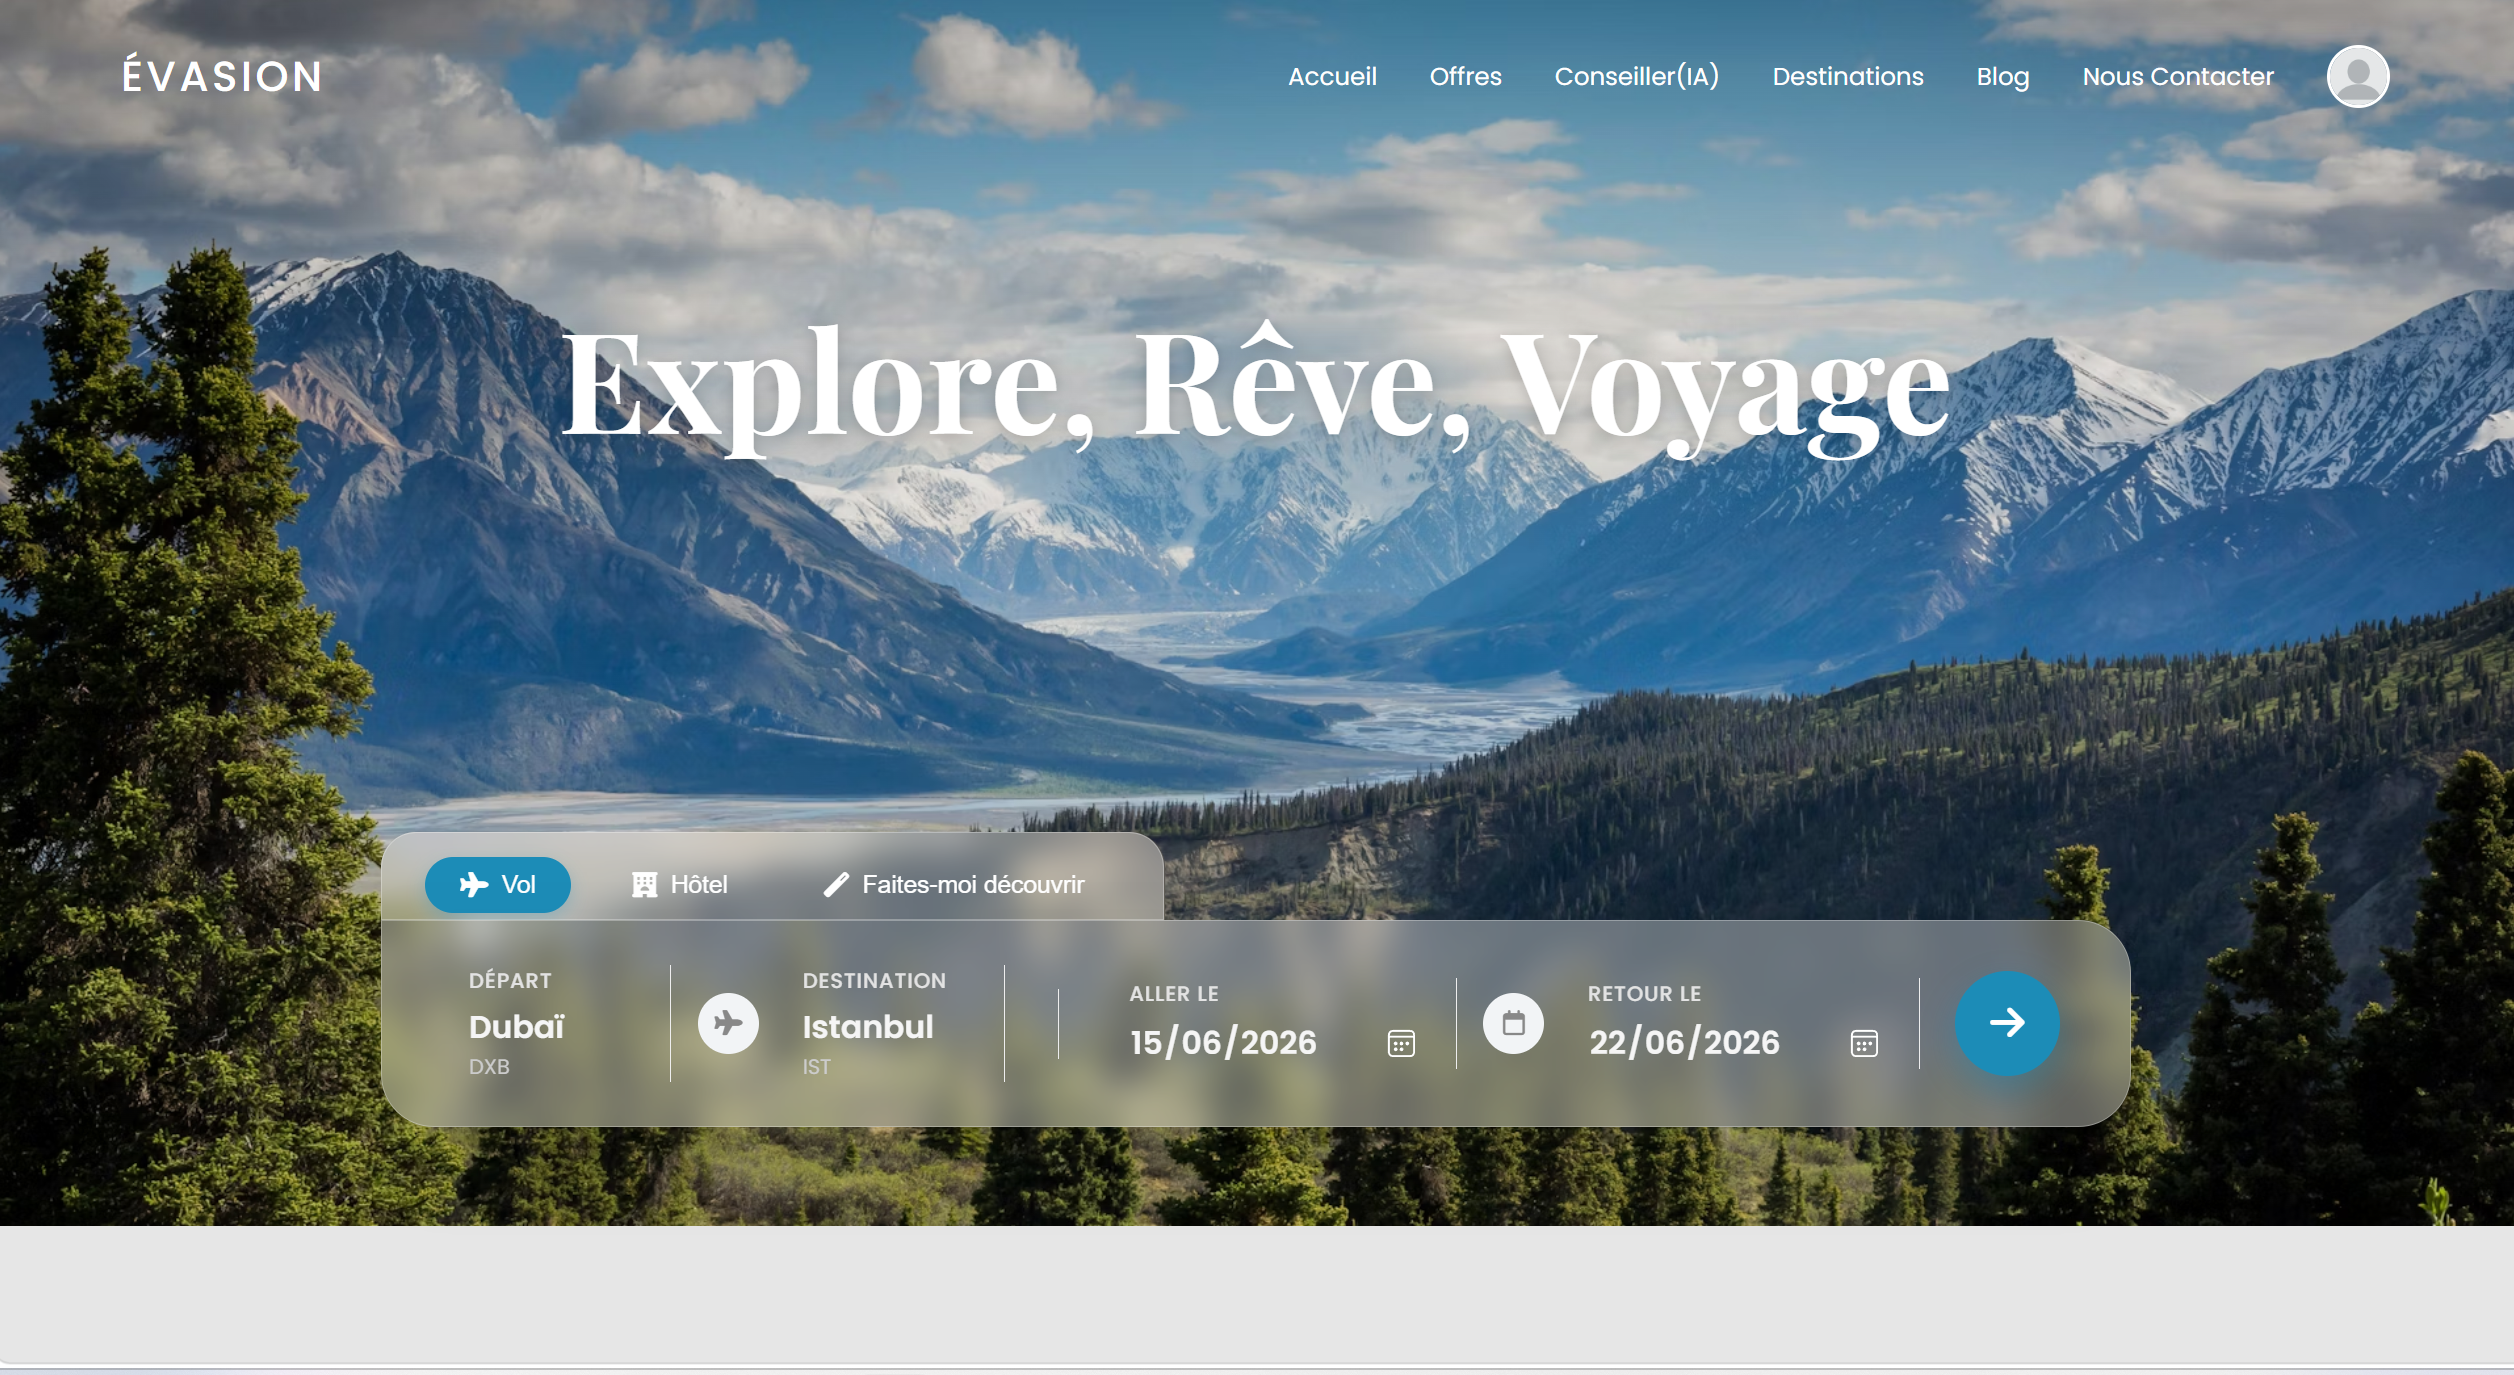
\includegraphics[width=\textwidth]{Capturedusite.png}
    \caption{Page d'accueil}
\end{figure}

\begin{figure}[H]
    \centering
    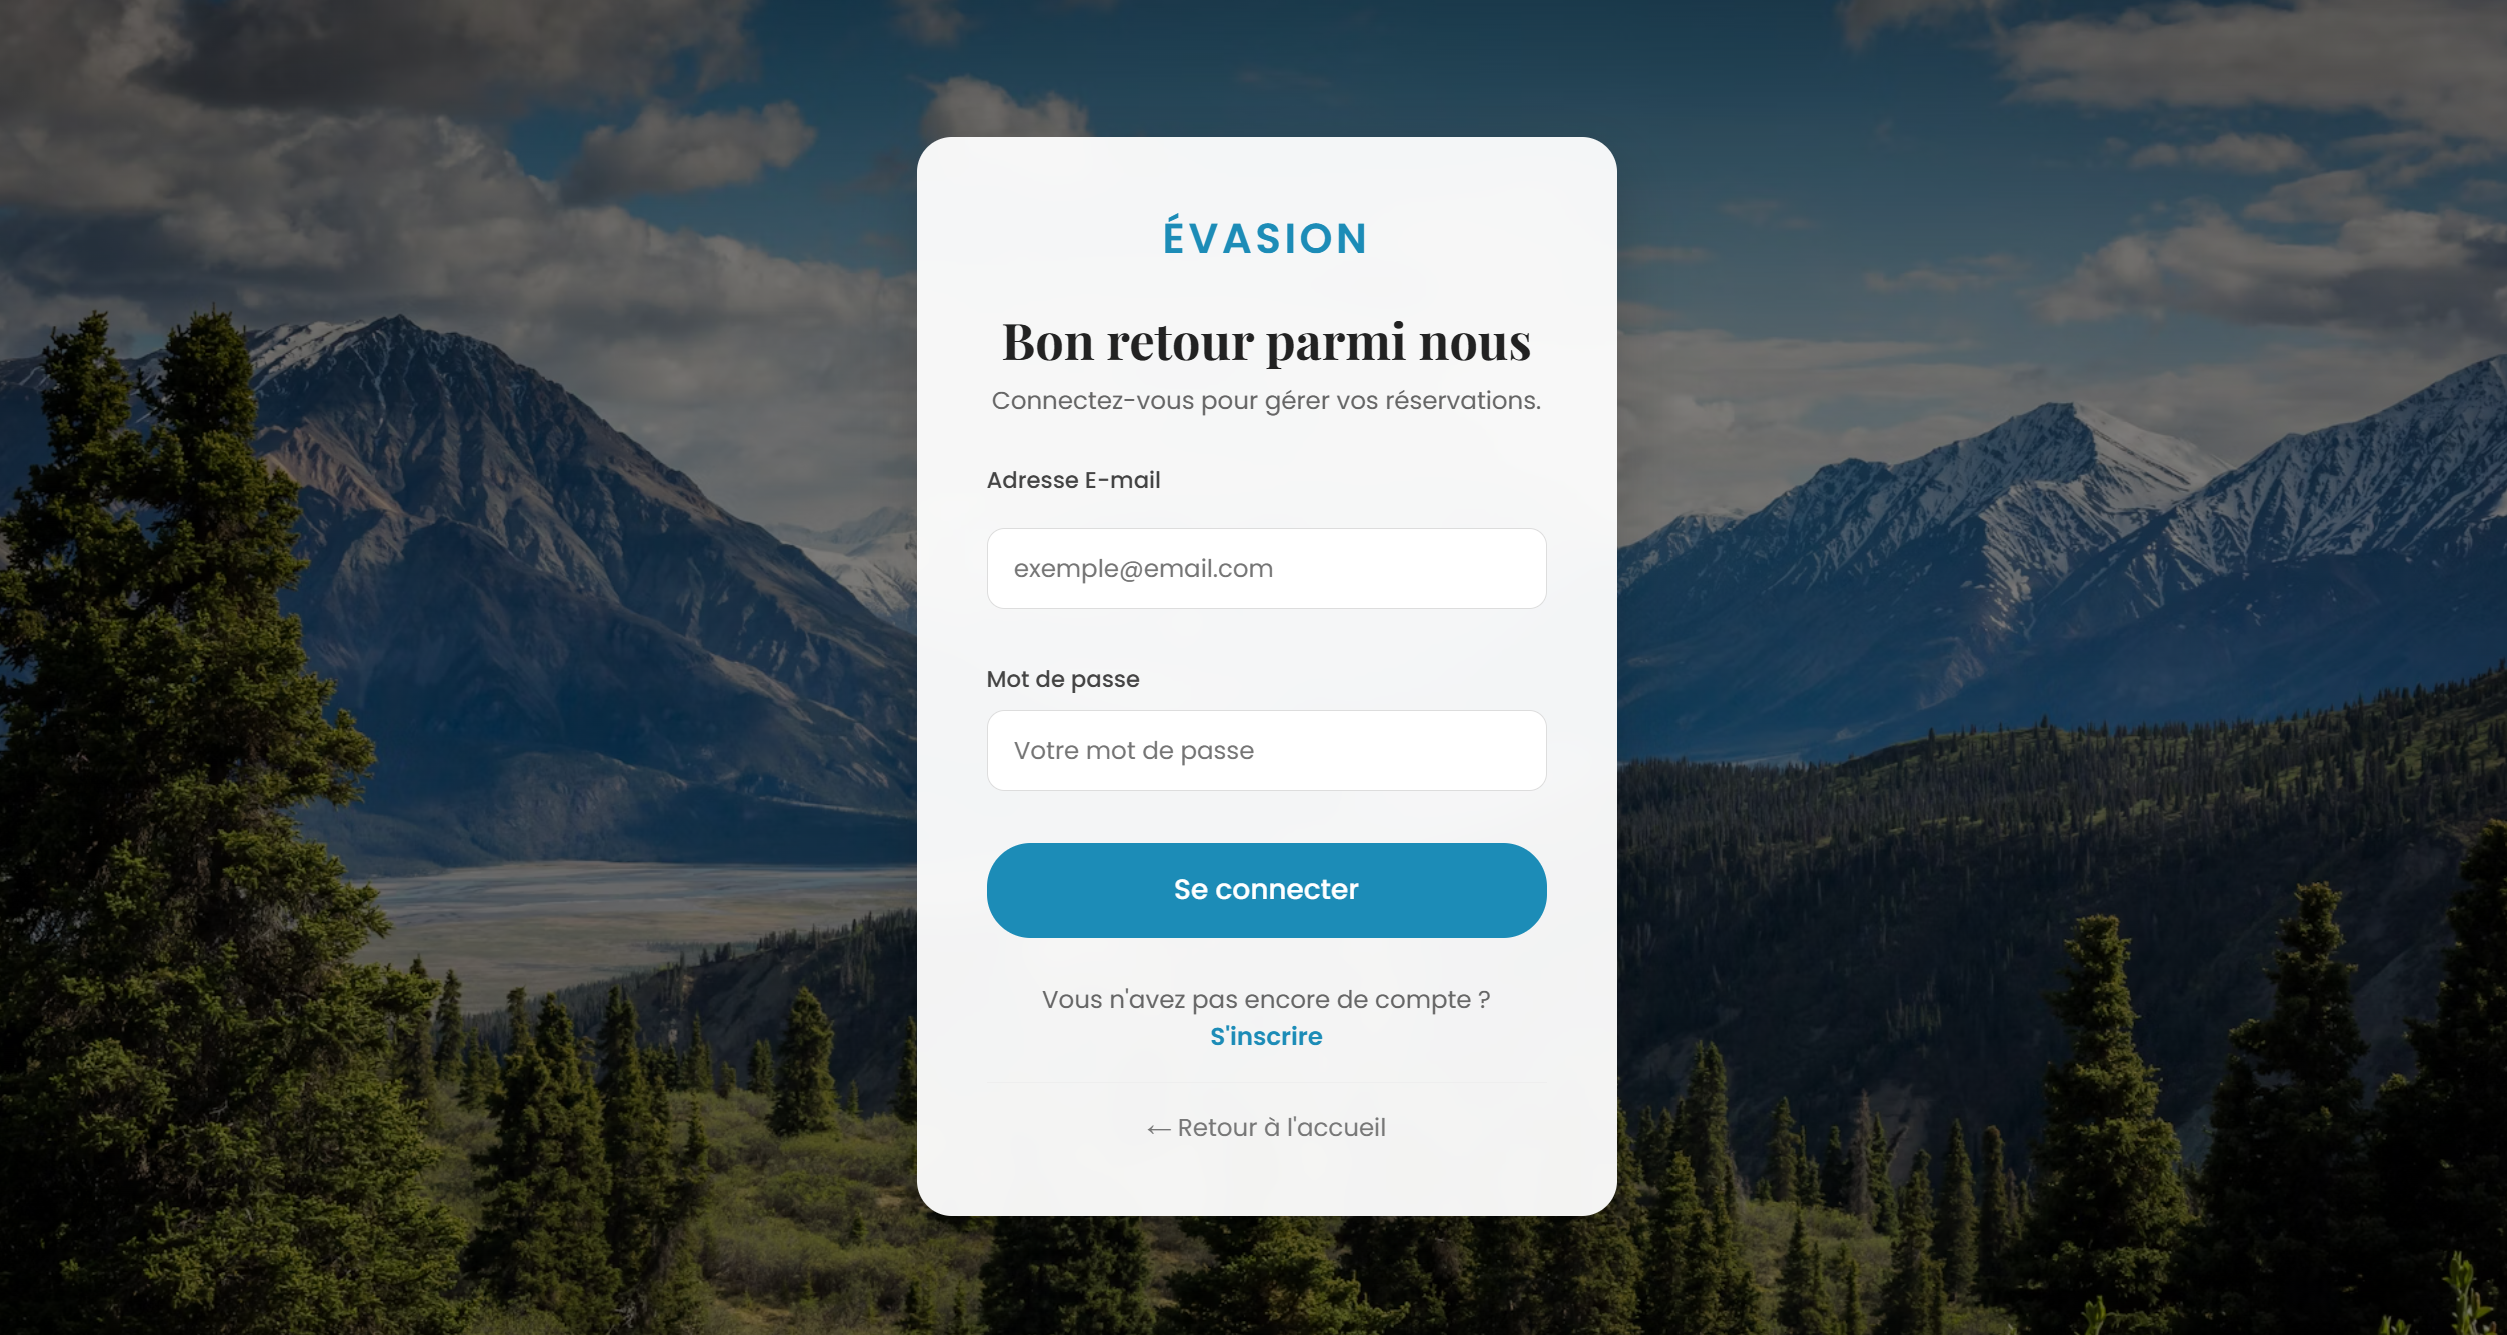
\includegraphics[width=\textwidth]{Capturedusite1.png}
    \caption{Page de connexion (\texttt{login.php})}
\end{figure}

\begin{figure}[H]
    \centering
    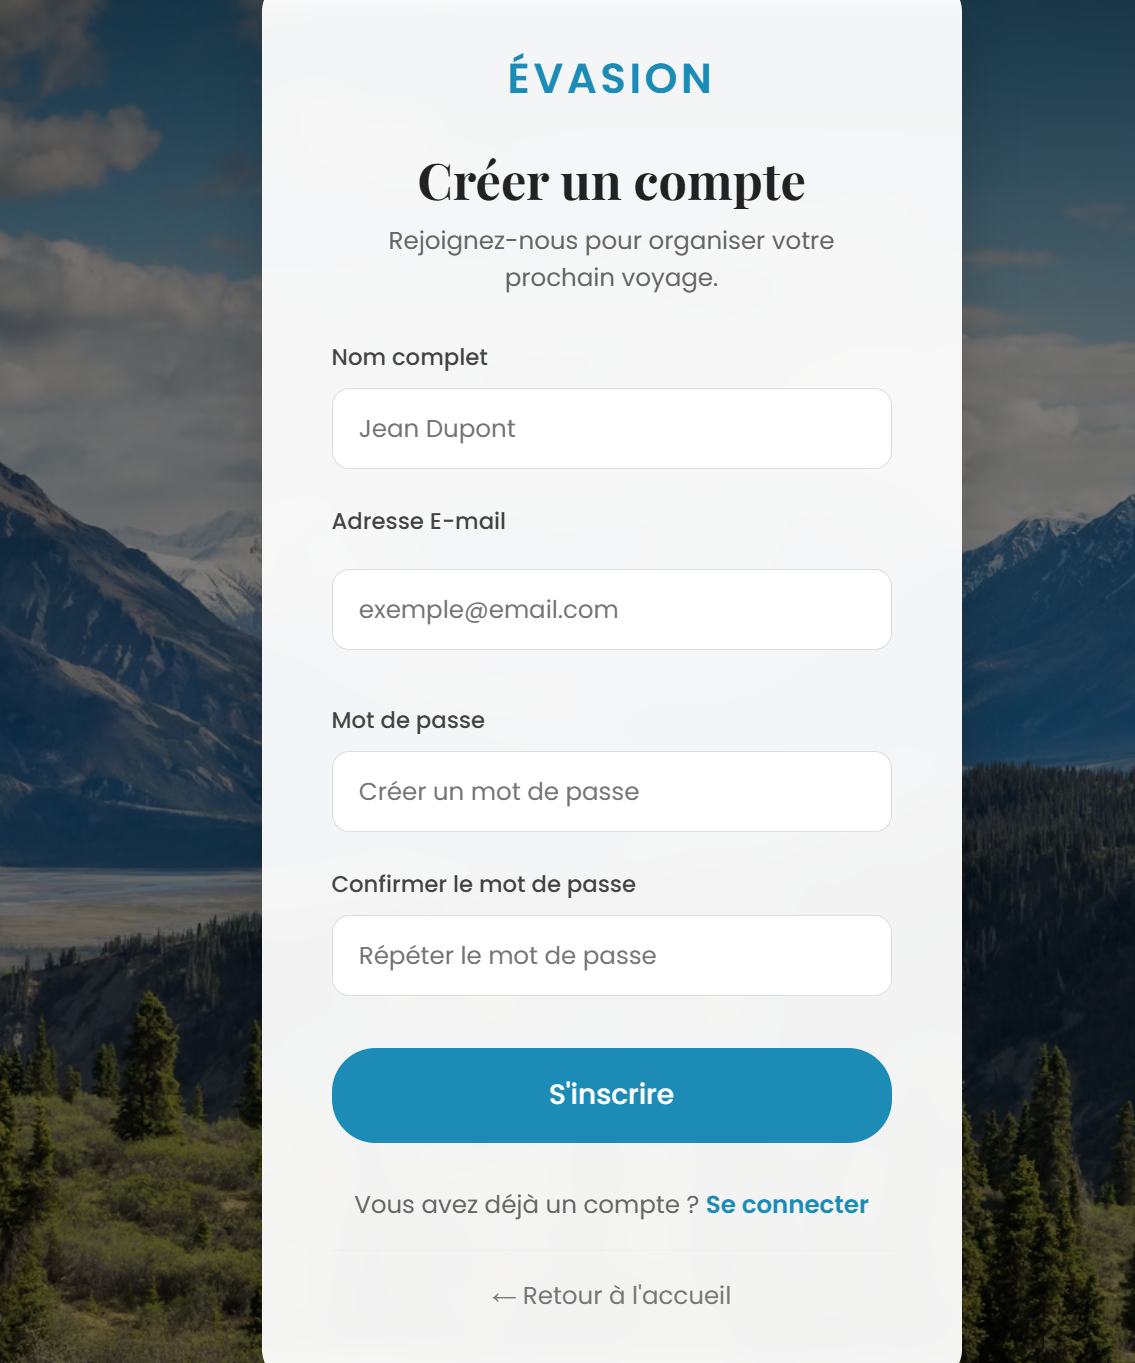
\includegraphics[width=\textwidth]{Inscription.png}
    \caption{Page d'inscription (\texttt{register.php})}
\end{figure}

\begin{figure}[H]
    \centering
    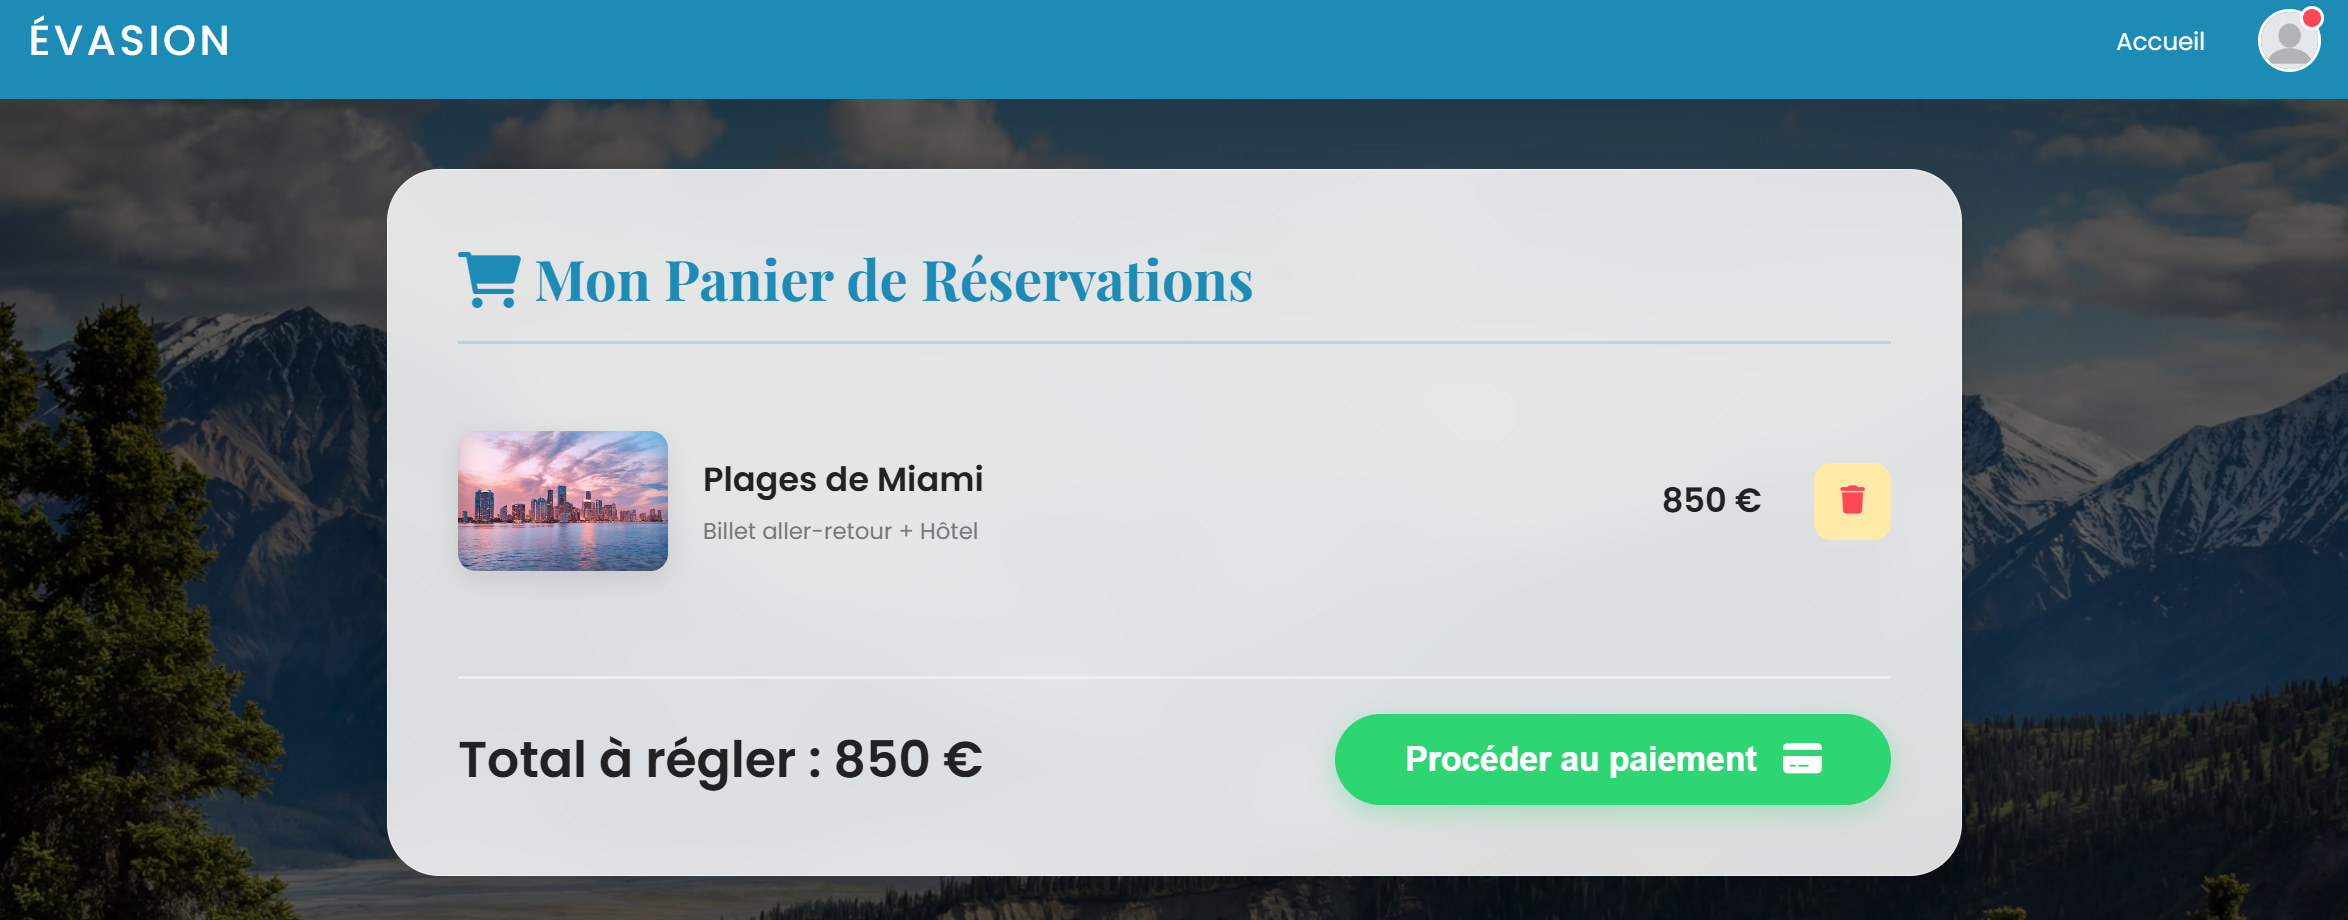
\includegraphics[width=\textwidth]{voyages.png}
    \caption{Page Mes Voyages (\texttt{voyages.php})}
\end{figure}

\begin{figure}[H]
    \centering
    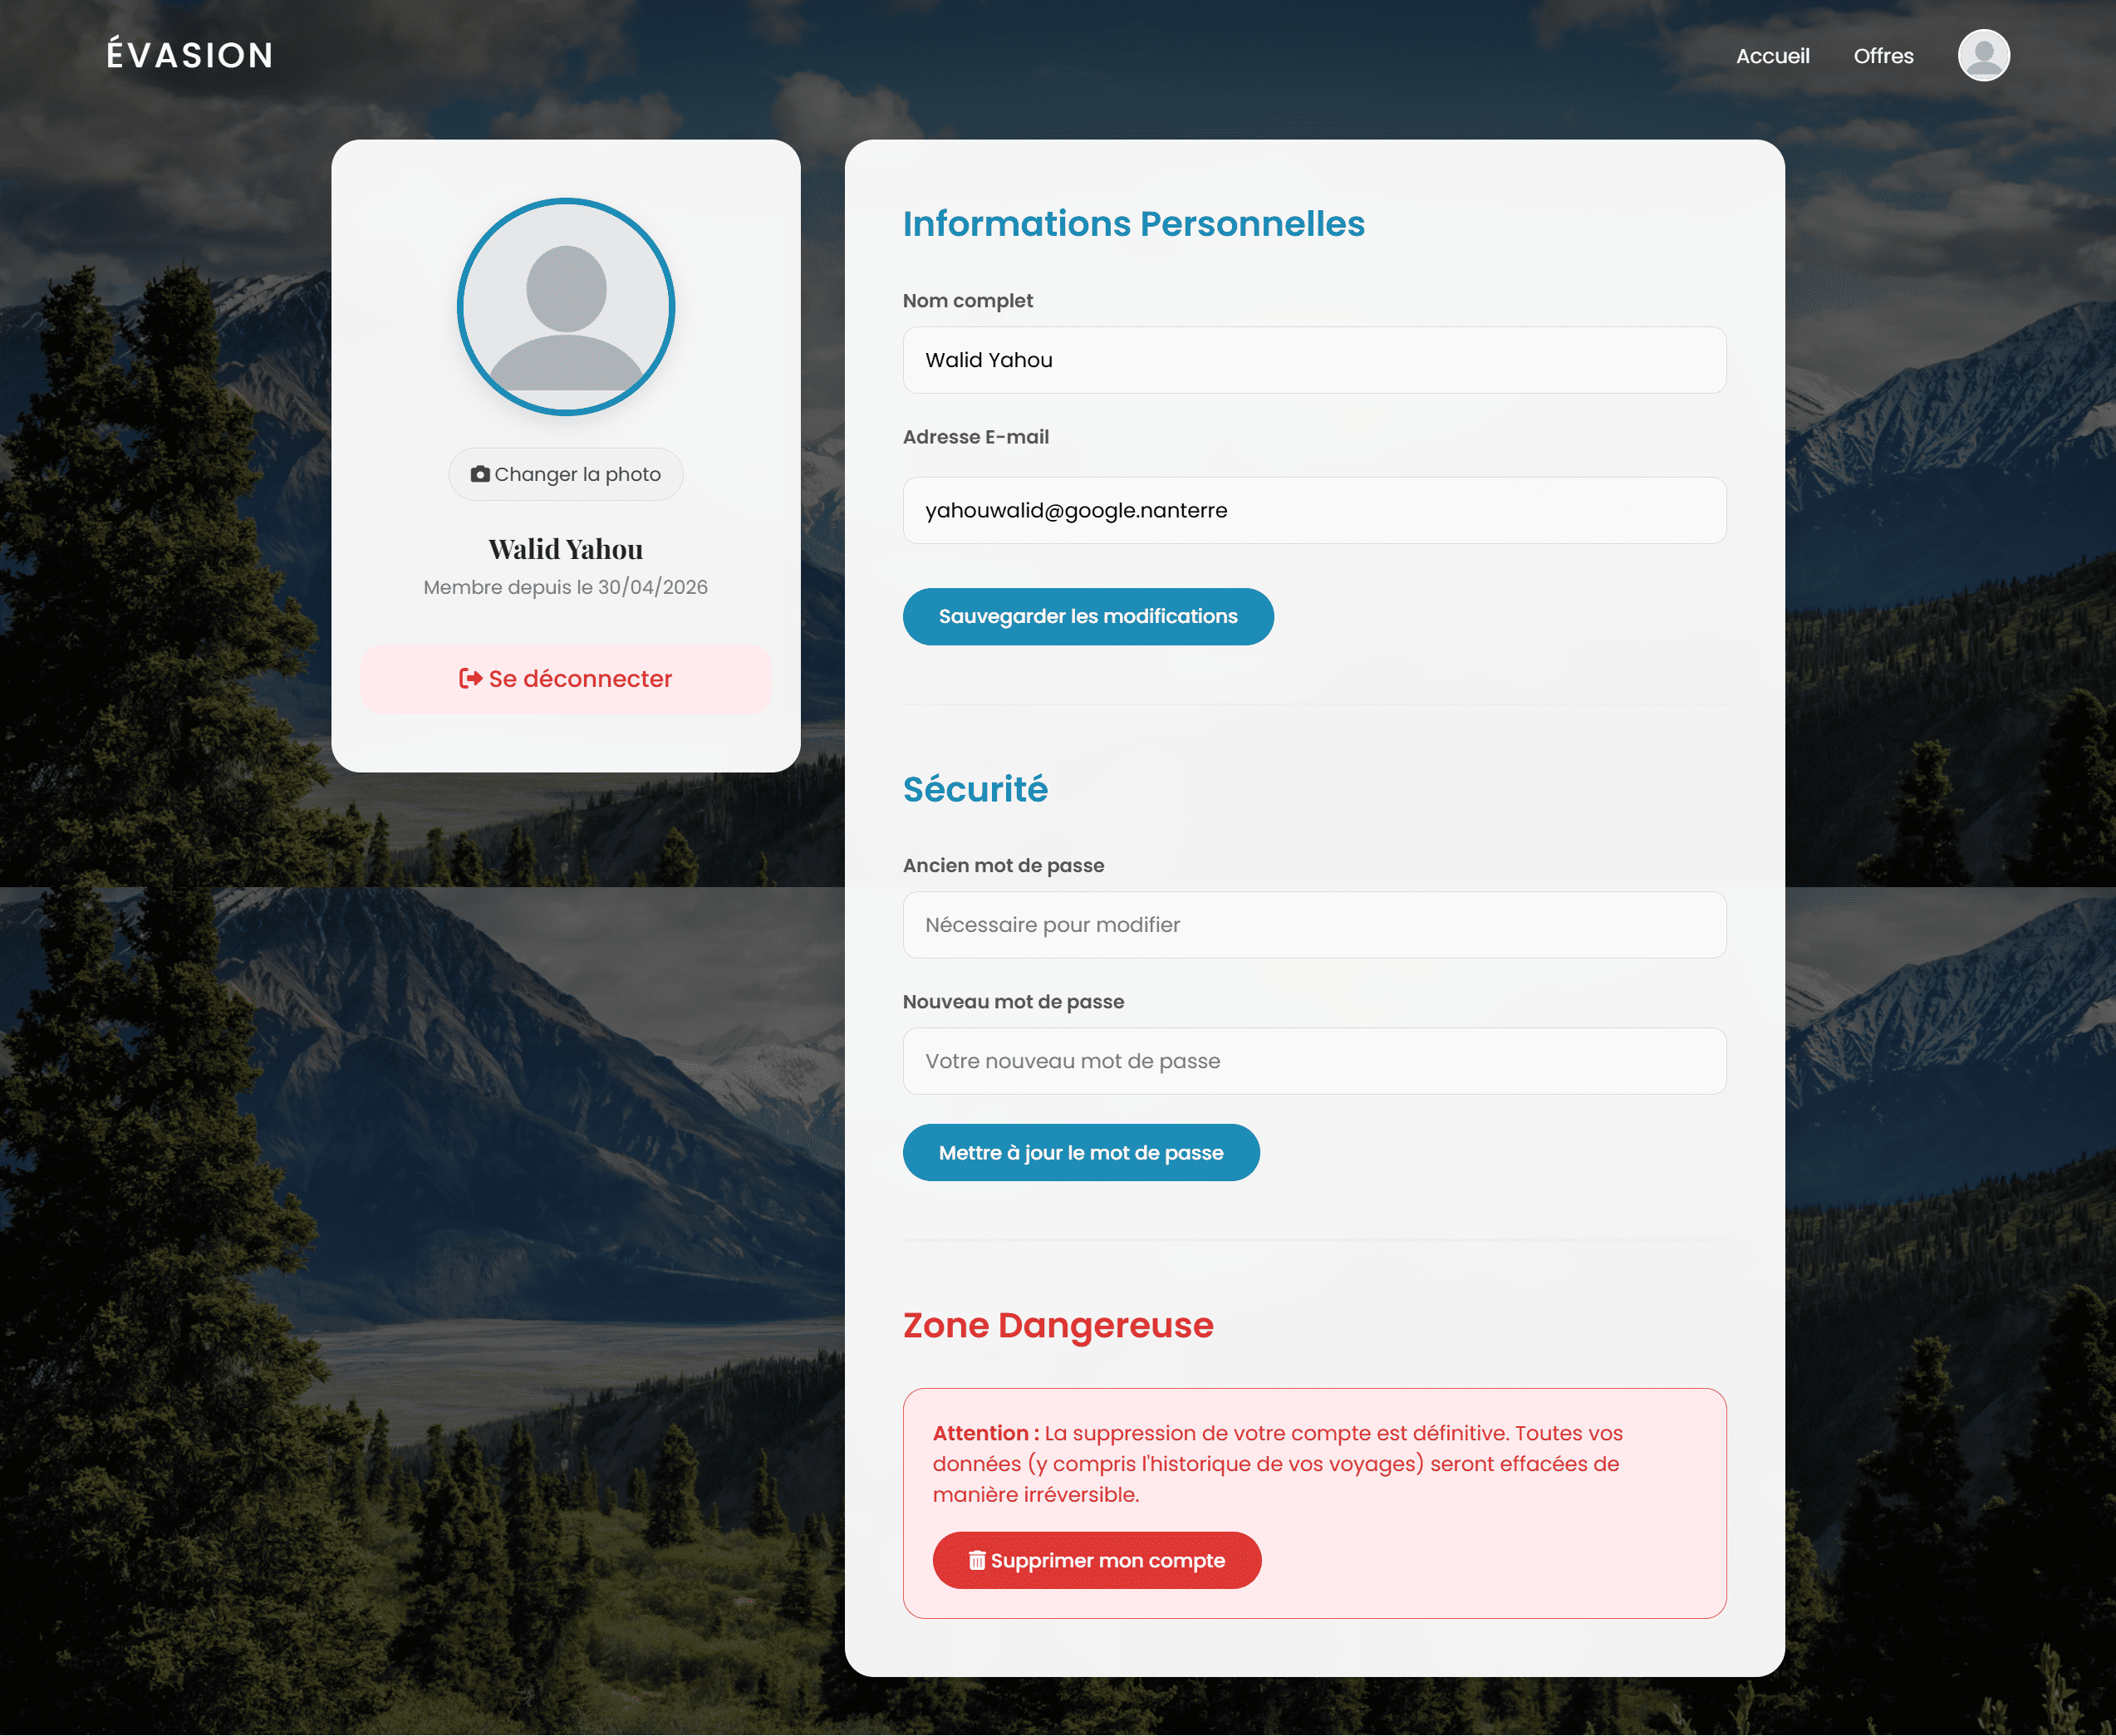
\includegraphics[width=\textwidth]{Screenshotprofil.png}
    \caption{Page Mon profil (\texttt{profil.php})}
\end{figure}

\begin{figure}[H]
    \centering
    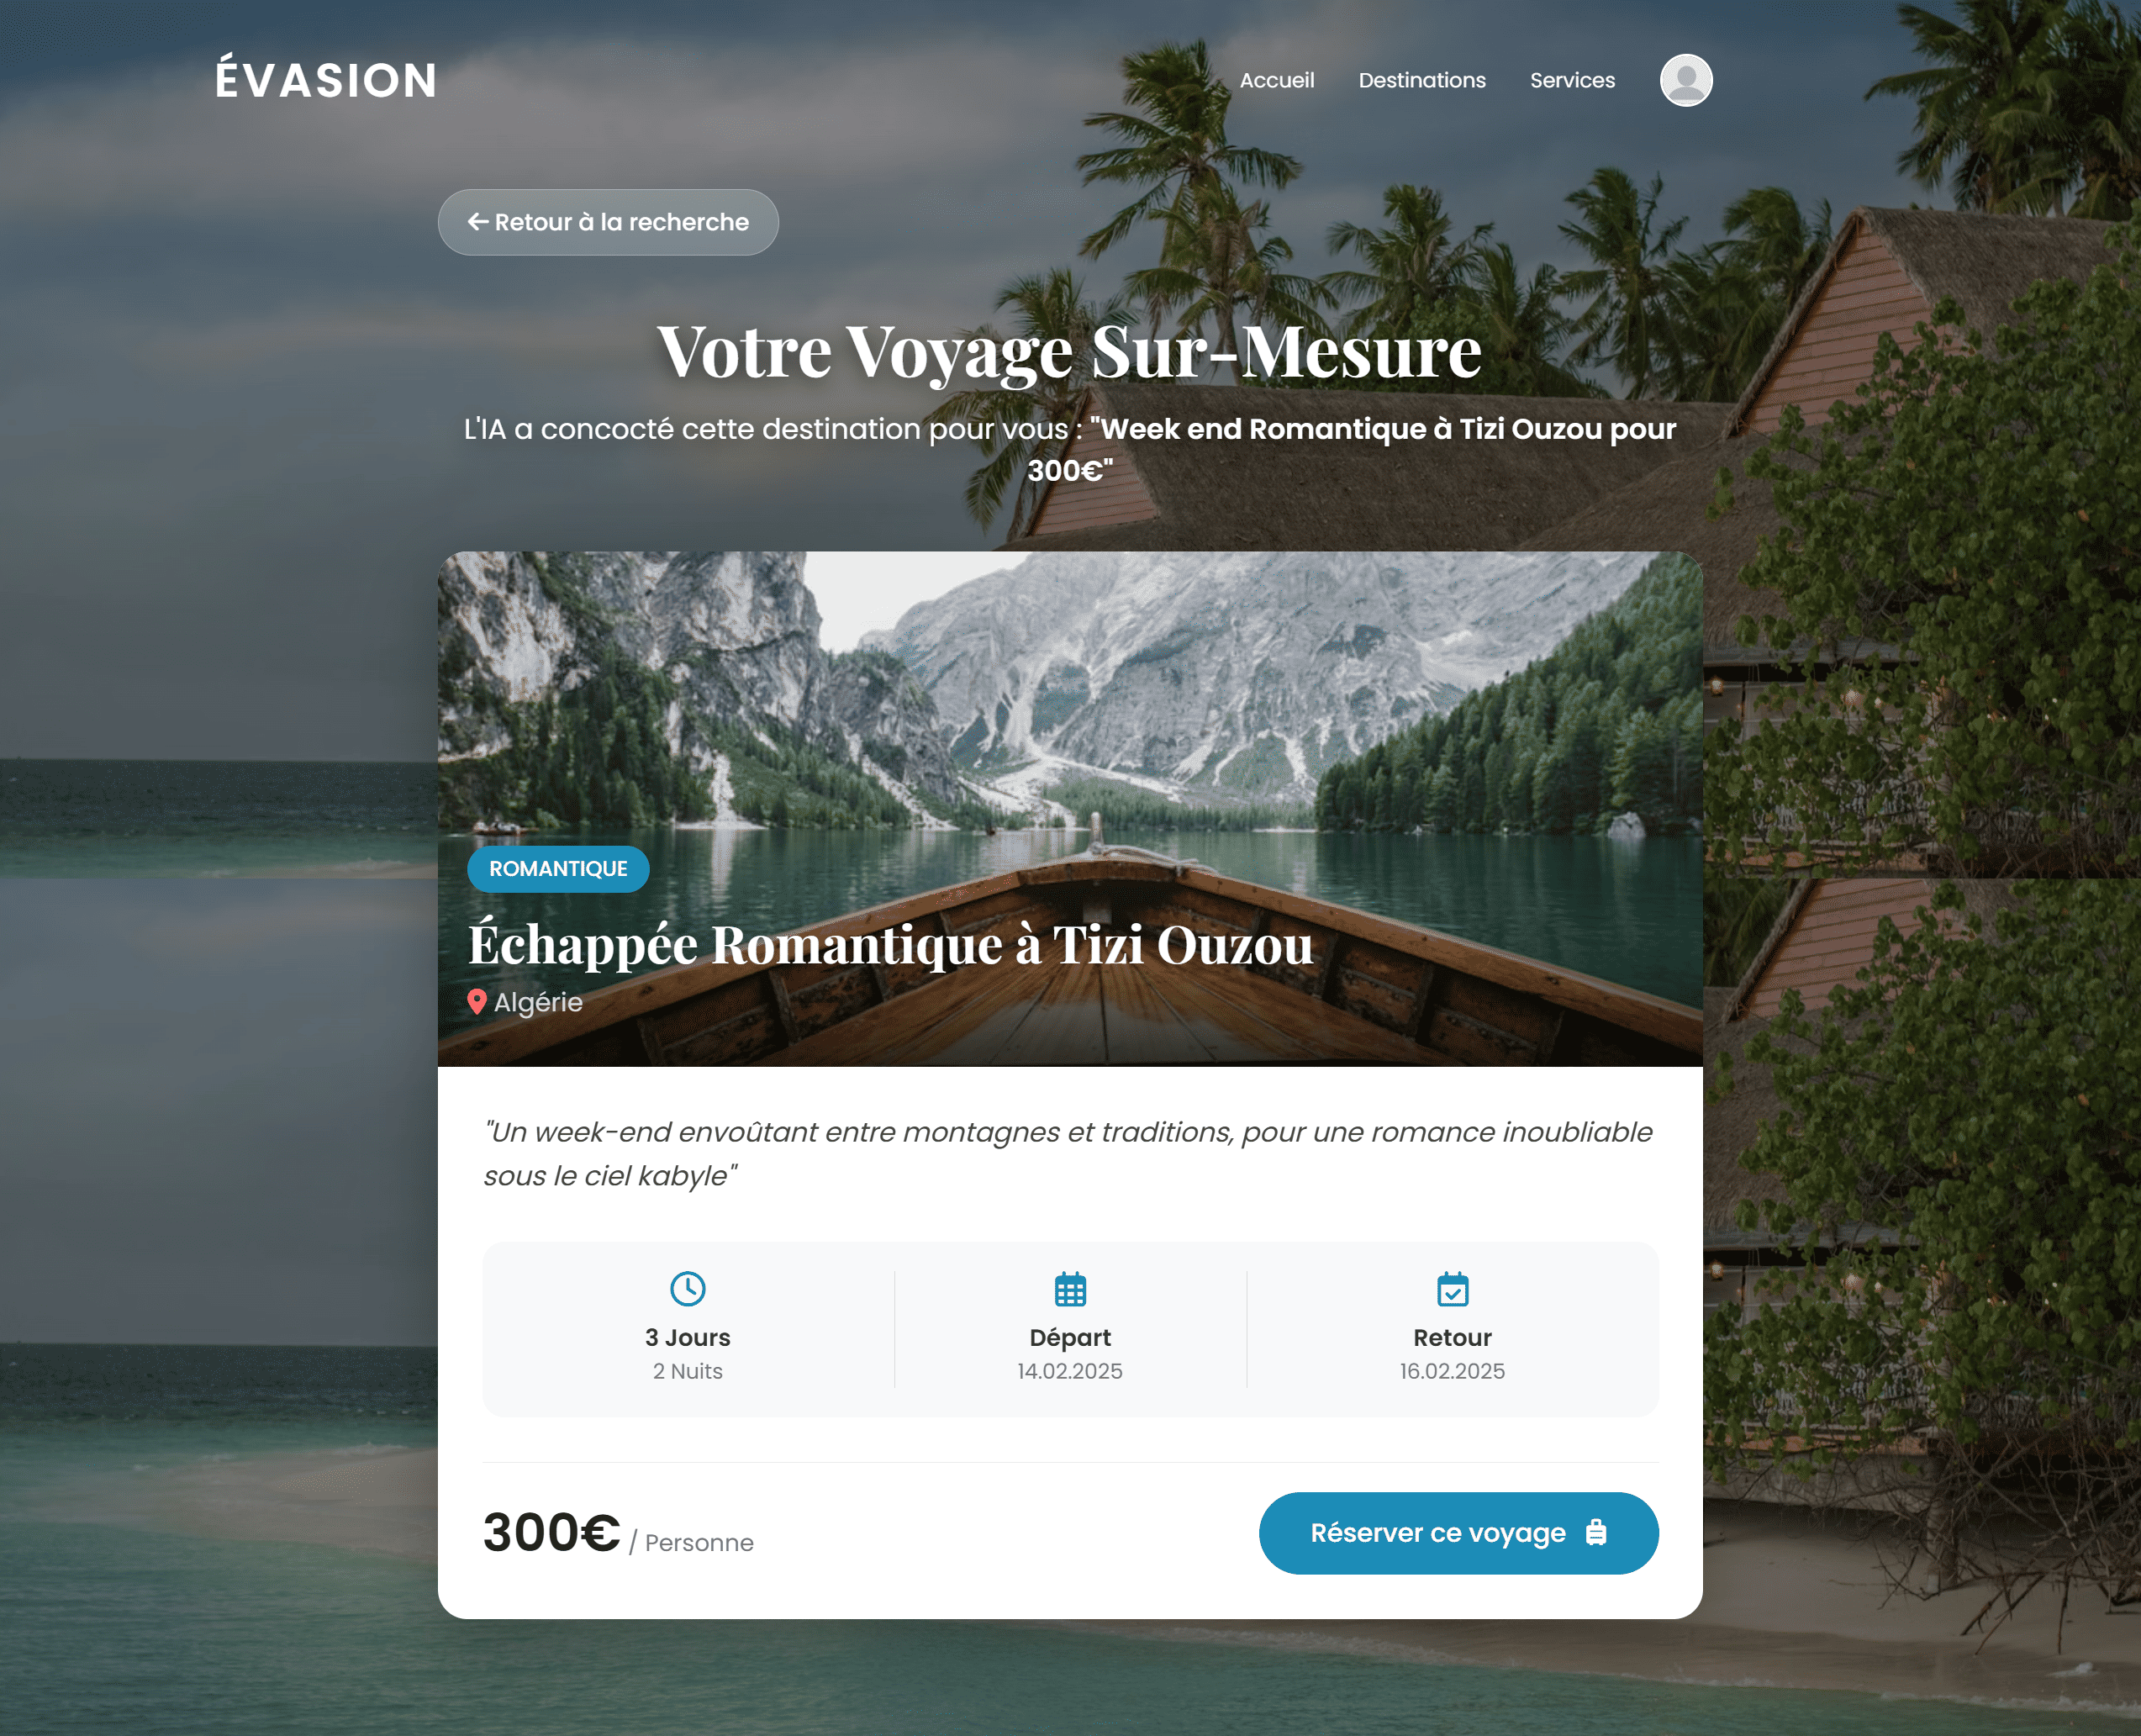
\includegraphics[width=\textwidth]{ScreenshotVoyage.png}
    \caption{Page Voyage généré par l'IA (\texttt{recherche\_ia.php})}
\end{figure}

\subsection{Identifiants de test}

Pour tester les fonctionnalités du site, les comptes suivants sont disponibles dans la base de données. \textbf{Attention :} Les mots de passe sont hachés pour des raisons de sécurité. Voici les identifiants en clair :

\begin{table}[H]
\centering
\begin{tabular}{|p{4cm}|p{5cm}|p{4cm}|}
\hline
\textbf{Email} & \textbf{Mot de passe} & \textbf{Rôle} \\
\hline
chat@chat.com & chat & Utilisateur \\
\hline
\end{tabular}
\caption{Comptes de test}
\end{table}

Pour créer un nouveau compte, utilisez le formulaire d'inscription (\texttt{register.php}).

% ---------------------------------------------------------
\section{Difficultés rencontrées}

Plusieurs difficultés techniques ont été rencontrées au cours du développement :

\begin{itemize}
  \item \textbf{Intégration de l'API Mistral AI} : la construction d'un prompt système rigoureux et le traitement de la réponse JSON ont demandé une gestion attentive du format attendu et des erreurs HTTP (codes 4xx/5xx) retournées par l'API.
  \item \textbf{Gestion des sessions PHP} : le panier de réservations étant stocké en session, il fallait synchroniser proprement les opérations d'ajout et de suppression sans créer de doublons lors des rechargements de page (résolu via \texttt{header("Location: ...")}).
  \item \textbf{Upload de fichiers} : création dynamique du dossier \texttt{uploads/}, validation des extensions et renommage unique des fichiers pour éviter les conflits entre utilisateurs.
  \item \textbf{Responsive design} : adapter l'interface à mobile avec le menu hamburger tout en maintenant une expérience cohérente (sous-menu profil, blocage du scroll arrière-plan).
  \item \textbf{Sécurité PDO} : passage de requêtes SQL brutes à des requêtes préparées sur l'ensemble des pages pour prévenir les injections.
\end{itemize}

% ---------------------------------------------------------
\section{Conclusion}

Ce projet nous a permis de mettre en pratique l'ensemble de la chaîne de développement web full-stack dans un contexte réaliste d'agence de voyages.

\textbf{Compétences acquises :}
\begin{itemize}
  \item Conception et interrogation d'une base de données relationnelle avec PHP PDO
  \item Gestion des sessions, de l'authentification et de la sécurisation des entrées
  \item Intégration d'une API d'intelligence artificielle (Mistral) dans un projet web
  \item Développement d'une interface responsive avec JavaScript vanilla
  \item Consommation d'une API externe (Open-Meteo) pour l'autocomplétion
\end{itemize}

\subsection{Améliorations possibles}

\begin{itemize}
  \item Remplacer le panier en session par une table SQL \texttt{reservations} pour persister les données entre les connexions.
  \item Ajouter un système de paiement simulé (Stripe Sandbox).
  \item Implémenter un espace d'administration complet (CRUD sur les destinations).
  \item Améliorer la pertinence du moteur IA en affinant le prompt système et en ajoutant un historique de conversation.
  \item Déployer le site sur un hébergement en ligne (OVH, Infomaniak, etc.).
\end{itemize}

% ---------------------------------------------------------
\section{Bibliographie}

\begin{itemize}
  \item Documentation PHP officielle : \url{https://www.php.net/docs.php}
  \item Documentation PDO : \url{https://www.php.net/manual/fr/book.pdo.php}
  \item API Mistral AI : \url{https://docs.mistral.ai/}
  \item API Open-Meteo Geocoding : \url{https://open-meteo.com/en/docs/geocoding-api}
  \item Documentation MariaDB : \url{https://mariadb.com/kb/fr/}
  \item MDN Web Docs (HTML/CSS/JS) : \url{https://developer.mozilla.org/fr/}
\end{itemize}

\end{document}